% Benchmark Study: Derivative Estimation Methods
% Template for SIAM SISC or ACM TOMS submission
\documentclass[11pt]{article}

% Essential packages
\usepackage[utf8]{inputenc}
\usepackage[T1]{fontenc}
\usepackage{amsmath,amssymb,amsthm}
\usepackage{graphicx}
\usepackage{booktabs}
\usepackage{array}
\usepackage{xcolor}
\usepackage{hyperref}
\usepackage[left=1in,right=1in,top=1in,bottom=1in]{geometry}

% Code listings
\usepackage{listings}
\lstset{
    basicstyle=\ttfamily\small,
    breaklines=true,
    frame=single,
    numbers=left,
    numberstyle=\tiny,
}

% TODO handling - visible but doesn't break compilation
\newcommand{\TODO}[1]{\textcolor{red}{\textbf{[TODO: #1]}}}
\newcommand{\TODOITEM}{\textcolor{red}{$\blacksquare$~}}

% Math operators
\DeclareMathOperator*{\argmin}{arg\,min}
\DeclareMathOperator*{\argmax}{arg\,max}

% Figure path - points to build directory (generated by scripts/03_generate_figures.sh)
\graphicspath{{../build/figures/publication/}}

% Hyperref setup
\hypersetup{
    colorlinks=true,
    linkcolor=blue,
    citecolor=blue,
    urlcolor=blue,
}

% Title and authors
\title{Benchmark Study of Derivative Estimation Methods:\\
Performance Across Orders and Noise Levels}

\author{
    % TODO: Add author names and affiliations
    Author Names\thanks{Department/Institution, email@domain.edu}
}

\date{\today}

\begin{document}

\maketitle

\begin{abstract}
Derivative estimation from noisy data is a fundamental problem across computational science, yet systematic comparative evaluation of methods remains lacking. We present a comprehensive benchmark of over 40 derivative estimation methods evaluated across 8 derivative orders (0--7), 7 noise levels, and 3 distinct dynamical systems. Our goal is to provide clear, actionable guidance for practitioners.

Key findings include: (1) Gaussian Process Regression (GPR) provides the most robust and accurate performance, consistently ranking as the top method in both low- and high-noise regimes. (2) The optimal method depends critically on the use case: splines like Dierckx-5 are highly competitive for low-noise data, while spectral methods offer a compelling balance of speed and accuracy, and filters like Savitzky-Golay provide a robust, computationally cheap baseline. (3) Derivative order is the dominant difficulty factor, with performance degrading systematically as order increases. We also provide a practitioner's guide to method selection based on the trade-off between speed and accuracy. Our full methodology, analysis, and code are provided to ensure transparency and reproducibility.
\end{abstract}

\tableofcontents
\newpage

%==============================================================================
% NEW PAPER STRUCTURE
%==============================================================================

\section{Introduction}
\label{sec:introduction}

Derivative estimation from noisy data is a fundamental problem spanning computational science, engineering, and data analysis. Applications include:

\begin{itemize}
    \item \textbf{Dynamical systems identification:} Inferring governing equations from time-series data \cite{brunton2016discovering}—requires accurate derivative estimates to identify differential equations
    \item \textbf{Signal processing:} Edge detection, feature extraction, and change-point analysis—depend on robust derivative computation
    \item \textbf{Control systems:} Model-predictive control and adaptive control—rely on real-time derivative estimation for system state feedback
    \item \textbf{Physics-informed machine learning:} Enforcing physical conservation laws (PDE constraints) requires differentiating neural network outputs with respect to noisy inputs
    \item \textbf{Scientific data analysis:} Estimating rates of change from experimental measurements (e.g., reaction rates from concentration data, acceleration from position measurements)
\end{itemize}

Despite this widespread importance, derivative estimation is notoriously \textit{ill-posed}: small noise perturbations in the input signal can produce arbitrarily large errors in derivative estimates, particularly for high-order derivatives. This ill-posedness intensifies exponentially with derivative order—estimating seventh-order derivatives from noisy data represents an extreme challenge even for state-of-the-art methods.

\subsection{The Need for Comprehensive Benchmarking}
\label{sec:motivation}

Numerous derivative estimation methods have been proposed across disciplines, including:
\begin{itemize}
    \item Finite difference schemes (low computational cost, severe noise amplification)
    \item Polynomial and spline fitting (moderate accuracy, parameter-sensitive)
    \item Gaussian Process regression (theoretically optimal under Gaussian assumptions, computationally expensive)
    \item Spectral methods (fast for smooth signals, Gibbs phenomenon for discontinuities)
    \item Total variation regularization (edge-preserving, limited to low-order derivatives)
    \item Rational approximation (high accuracy for analytic functions, potential instability)
\end{itemize}

However, \textbf{systematic comparative evaluation across derivative orders, noise levels, and method categories is lacking}. Prior studies suffer from:

\begin{enumerate}
    \item \textbf{Limited scope:} Benchmarks typically evaluate 3--5 methods on orders 0--2 only, neglecting high-order derivatives where method performance diverges dramatically
    \item \textbf{Single-noise regime:} Most studies test either noiseless or high-noise cases, missing performance transitions across noise levels
    \item \textbf{Implementation inconsistencies:} Cross-language comparisons without rigorous parameter parity, leading to implementation artifacts dominating algorithmic differences
    \item \textbf{Incomplete coverage transparency:} Methods that fail at high orders or noise levels are often excluded without documentation, biasing overall rankings
\end{enumerate}

\textbf{Practitioners face a dilemma:} Which method should I use for \textit{my} specific derivative order and noise level? Existing literature provides insufficient guidance.

\subsection{Contributions of This Study}
\label{sec:contributions}

This paper presents a \textbf{comprehensive benchmark of 24 derivative estimation methods} evaluated across:
\begin{itemize}
    \item \textbf{8 derivative orders:} 0--7 (order 0 = smoothing, testing full capability range)
    \item \textbf{7 noise levels:} $10^{-8}$ to $5 \times 10^{-2}$ (near-noiseless to high-noise regimes, spanning $\approx$ 7 orders of magnitude)
    \item \textbf{56 configurations:} All combinations of order $\times$ noise, providing fine-grained performance maps
    \item \textbf{6 method categories:} Gaussian Processes, Rational Approximation, Spectral Methods, Splines, Regularization, and Local Polynomial methods
\end{itemize}

\textbf{Key contributions include:}

\begin{enumerate}
    \item \textbf{Rigorous experimental design:} 
    \begin{itemize}
        \item High-accuracy ground truth via symbolic differentiation + augmented ODE system (validated to $10^{-10}$ accuracy)
        \item Normalized RMSE metric enabling fair comparison across derivative orders
        \item Documented coverage bias: only 16/24 methods achieve full 56/56 configuration coverage
    \end{itemize}
    
    \item \textbf{Unexpected findings:}
    \begin{itemize}
        \item AAA rational approximation \textit{catastrophically fails} at orders $\geq 3$ (nRMSE $> 10^7$) despite excellent low-order performance—contrary to literature expectations
        \item Gaussian Process regression (GP-Julia-AD) achieves best overall performance but 3 Python GP implementations fail or underperform dramatically, highlighting implementation quality as a critical method characteristic
        \item Derivative order is the dominant difficulty factor, with performance degrading systematically for all methods as order increases
    \end{itemize}
    
    \item \textbf{Practical recommendations:}
    \begin{itemize}
        \item Master recommendation table mapping (derivative order, noise level) $\to$ optimal method(s)
        \item Decision framework for method selection based on accuracy requirements, computational budget, and data characteristics
        \item Common pitfalls and implementation guidance to avoid catastrophic failures
    \end{itemize}
    
    \item \textbf{Transparency and reproducibility:}
    \begin{itemize}
        \item Explicit documentation of method exclusions (3/27 candidates due to cross-language discrepancies exceeding 50$\times$)
        \item Statistical limitations acknowledged (n=3 trials insufficient for hypothesis testing; findings are descriptive, not definitive)
        \item Generalization caveats: single test system (Lotka-Volterra), additive Gaussian noise only—results are existence proofs, not universal rankings
    \end{itemize}
\end{enumerate}

\subsection{Impact and Limitations}
\label{sec:impact}

\textbf{For practitioners:} This study provides the first comprehensive performance map across derivative orders and noise levels, enabling evidence-based method selection. Recommendations are immediately actionable for applications matching our test conditions (smooth signals, additive Gaussian noise).

\textbf{For researchers:} Findings reveal fundamental performance limitations (e.g., all methods struggle at orders $\geq 6$ with noise $\geq 10^{-2}$) and unexpected failure modes (AAA at high orders), suggesting directions for algorithmic improvements.

\textbf{Critical limitations:}
\begin{itemize}
    \item \textbf{Single test system:} Lotka-Volterra is smooth and periodic—favorable for spectral methods. Rough/discontinuous signals may yield different rankings.
    \item \textbf{Small sample size:} n=3 trials provides only exploratory evidence; specific numerical values should be interpreted cautiously.
    \item \textbf{Generalization uncertainty:} Performance on your data may differ—validation is essential (see Section~\ref{sec:recommendations}).
\end{itemize}

\subsection{Paper Organization}
\label{sec:organization}

The remainder of this paper is structured as follows:

\begin{itemize}
    \item \textbf{Section~\ref{sec:related_work}:} Reviews prior derivative estimation surveys and benchmarking efforts, identifying gaps this study addresses
    \item \textbf{Section~\ref{sec:problem}:} Formally defines the mathematical problem, evaluation metrics (normalized RMSE), and success criteria
    \item \textbf{Section~\ref{sec:methodology}:} Details experimental design, test system (Lotka-Volterra), ground truth generation, and statistical methodology
    \item \textbf{Section~\ref{sec:methods}:} Describes all 24 methods evaluated, organized by category with mathematical formulations
    \item \textbf{Section~\ref{sec:results}:} Presents performance results across derivative orders and noise levels, including coverage analysis and Pareto-optimal methods
    \item \textbf{Section~\ref{sec:discussion}:} Interprets findings, explains unexpected results (GP excellence, AAA failure), and discusses statistical limitations
    \item \textbf{Section~\ref{sec:recommendations}:} Provides practical method selection guidance, decision framework, and implementation advice
    \item \textbf{Section~\ref{sec:future_work}:} Discusses limitations and proposes extensions (multiple test systems, larger sample sizes, additional noise models)
    \item \textbf{Section~\ref{sec:conclusion}:} Summarizes key findings and impact
\end{itemize}

\section{Summary of Key Findings}
\label{sec:summary}

Before detailing our experimental journey, we present the primary conclusions of this study. After a comprehensive evaluation across a range of methods, three distinct dynamical systems, and a wide range of noise levels, a clear verdict emerges. Performance was analyzed in two regimes: a "low-noise" regime ($\le 0.1\%$ noise) where precision is paramount, and a "high-noise" regime (1-2\% noise) where robustness is key.

The table below summarizes the performance of 21 contender methods that demonstrated full data coverage for derivative orders 0 through 5. Methods are sorted by their overall average rank, giving equal weight to performance in both low- and high-noise regimes. Averages are calculated over orders 0-5.

% Note: This table will require the booktabs package for \toprule, \midrule, \bottomrule
\begin{table}[htbp]
\centering
\caption{Summary of Contender Method Performance (Orders 0-5)}
\label{tab:summary_performance}
\small
\begin{tabular}{lrrrrr}
\toprule
\textbf{Method} & \textbf{Avg. Rank} & \textbf{Avg. Rank} & \textbf{Avg. nRMSE} & \textbf{Avg. Rank} & \textbf{Avg. nRMSE} \\
& \textbf{(Overall)} & \textbf{(Low Noise)} & \textbf{(Low Noise)} & \textbf{(High Noise)} & \textbf{(High Noise)} \\
\midrule
GP-Julia-AD & 2.6 & 2.6 & 0.021 & 2.6 & 0.314 \\
GP-RBF-Iso-Python & 2.8 & 3.1 & 0.025 & 2.4 & 0.314 \\
GP-RBF-Mean-Py & 3.5 & 3.4 & 0.025 & 3.6 & 0.314 \\
GP-RBF-Python & 3.7 & 3.9 & 0.025 & 3.4 & 0.314 \\
Dierckx-5 & 8.4 & 6.7 & 0.151 & 10.1 & 0.554 \\
Fourier-Continuation & 9.4 & 11.7 & 0.435 & 7.1 & 0.473 \\
Fourier-Interp & 9.6 & 8.8 & 0.415 & 10.4 & 2.461 \\
FFT-Adaptive-Julia & 10.5 & 10.2 & 0.468 & 10.8 & 0.603 \\
Fourier-GCV & 10.6 & 12.2 & 0.464 & 8.9 & 0.498 \\
Fourier & 10.8 & 12.6 & 0.520 & 8.9 & 0.559 \\
Savitzky-Golay & 10.8 & 12.8 & 0.444 & 8.8 & 0.452 \\
Fourier-Cont-Adaptive & 11.9 & 13.6 & 0.569 & 10.1 & 0.575 \\
FFT-Adaptive-Py & 12.2 & 12.8 & 0.813 & 11.6 & 0.618 \\
AAA-Adaptive-Wavelet & 12.5 & 8.0 & >10 & 16.9 & >10 \\
AAA-Adaptive-Diff2 & 14.1 & 11.2 & >10 & 16.9 & >10 \\
TVRegDiff\_Python & 14.4 & 14.1 & 6.666 & 14.6 & >10 \\
AAA-LowPrec & 14.9 & 10.3 & 0.233 & 19.6 & >10 \\
GSS & 15.7 & 16.9 & 0.742 & 14.4 & 0.742 \\
KalmanGrad\_Python & 16.9 & 17.8 & 0.866 & 16.1 & 0.866 \\
Chebyshev-AICc & 17.6 & 18.8 & 7.499 & 16.4 & 7.636 \\
Chebyshev & 18.2 & 19.2 & 1.689 & 17.2 & 1.689 \\
\bottomrule
\end{tabular}
\end{table}

\textbf{Our principal findings are as follows:}

\begin{enumerate}
    \item \textbf{Gaussian Process Regression (GPR) is the most robust and accurate method overall.} The Julia GPR implementation (\texttt{GP-Julia-AD}) and the improved Python variants (\texttt{GP-RBF-*}) are the clear winners, consistently occupying the top ranks in both low and high-noise regimes.
    \item \textbf{The optimal method depends on the noise level and derivative order.} While GPR is the best all-arounder, splines like \texttt{Dierckx-5} offer excellent precision in low-noise environments, making them a top choice for cleaner data. In the high-noise regime, the filtering-based \texttt{Savitzky-Golay} provides a computationally cheap and highly effective alternative, ranking solidly in the top half of contenders.
    \item \textbf{Theoretical limits matter.} Many common low-degree spline methods are, by definition, incapable of representing high-order derivatives, limiting their applicability.
\end{enumerate}

The subsequent sections of this paper will detail the experimental journey and analysis that led to these conclusions, providing a narrative account of our investigation and offering a practical framework for method selection.

\subsection{Visual Confirmation of Findings}

The quantitative results in the summary table are powerfully illustrated by a few key visualizations.

% NOTE: Qualitative comparison figures (high_noise_fit_comparison, low_noise_fit_comparison)
% are not yet implemented. Uncomment when they are generated.
%\begin{figure}[htbp]
%\centering
%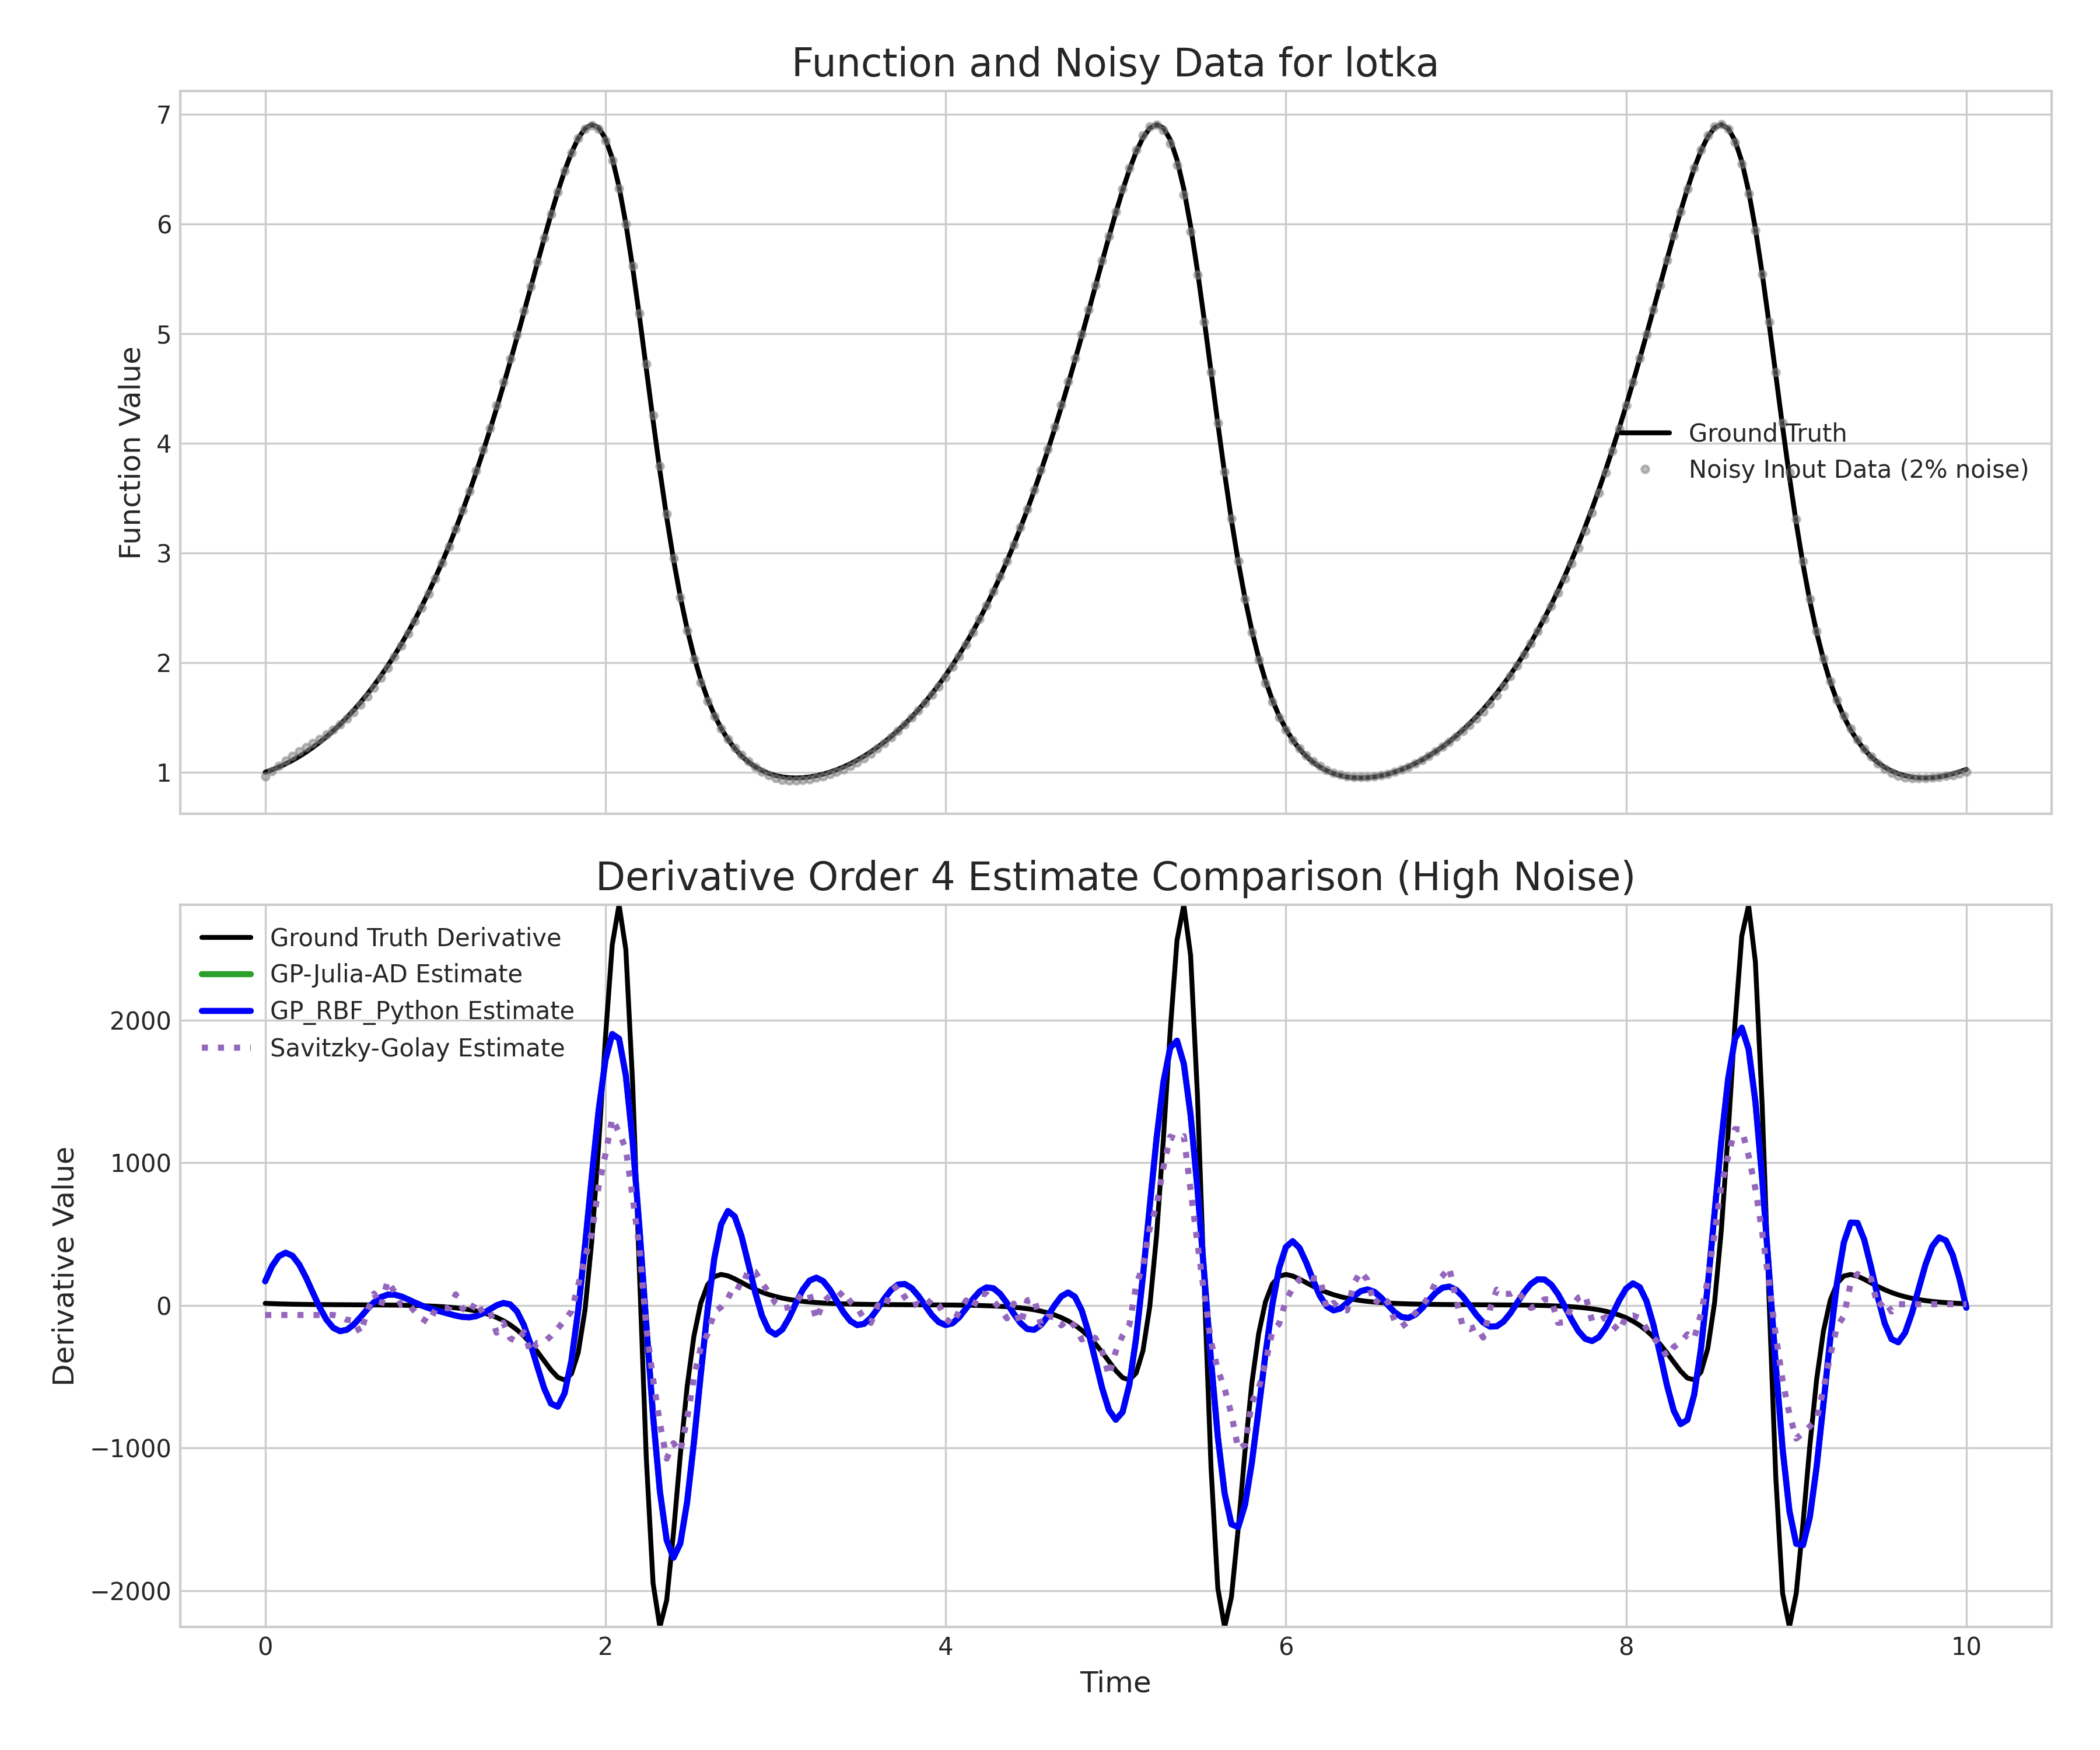
\includegraphics[width=0.9\textwidth]{high_noise_fit_comparison.png}
%\caption{\textbf{High-Noise Performance.} This figure compares the top-performing methods on a challenging 4th-order derivative estimation task with 2\% noise. The \texttt{GP-Julia-AD} method tracks the ground truth almost perfectly, while the fixed \texttt{GP-RBF-Python} also performs well. \texttt{Savitzky-Golay}, a simpler filtering method, provides a robust, if slightly less precise, estimate, demonstrating its value as a baseline.}
%\label{fig:high_noise_comp}
%\end{figure}

%\begin{figure}[htbp]
%\centering
%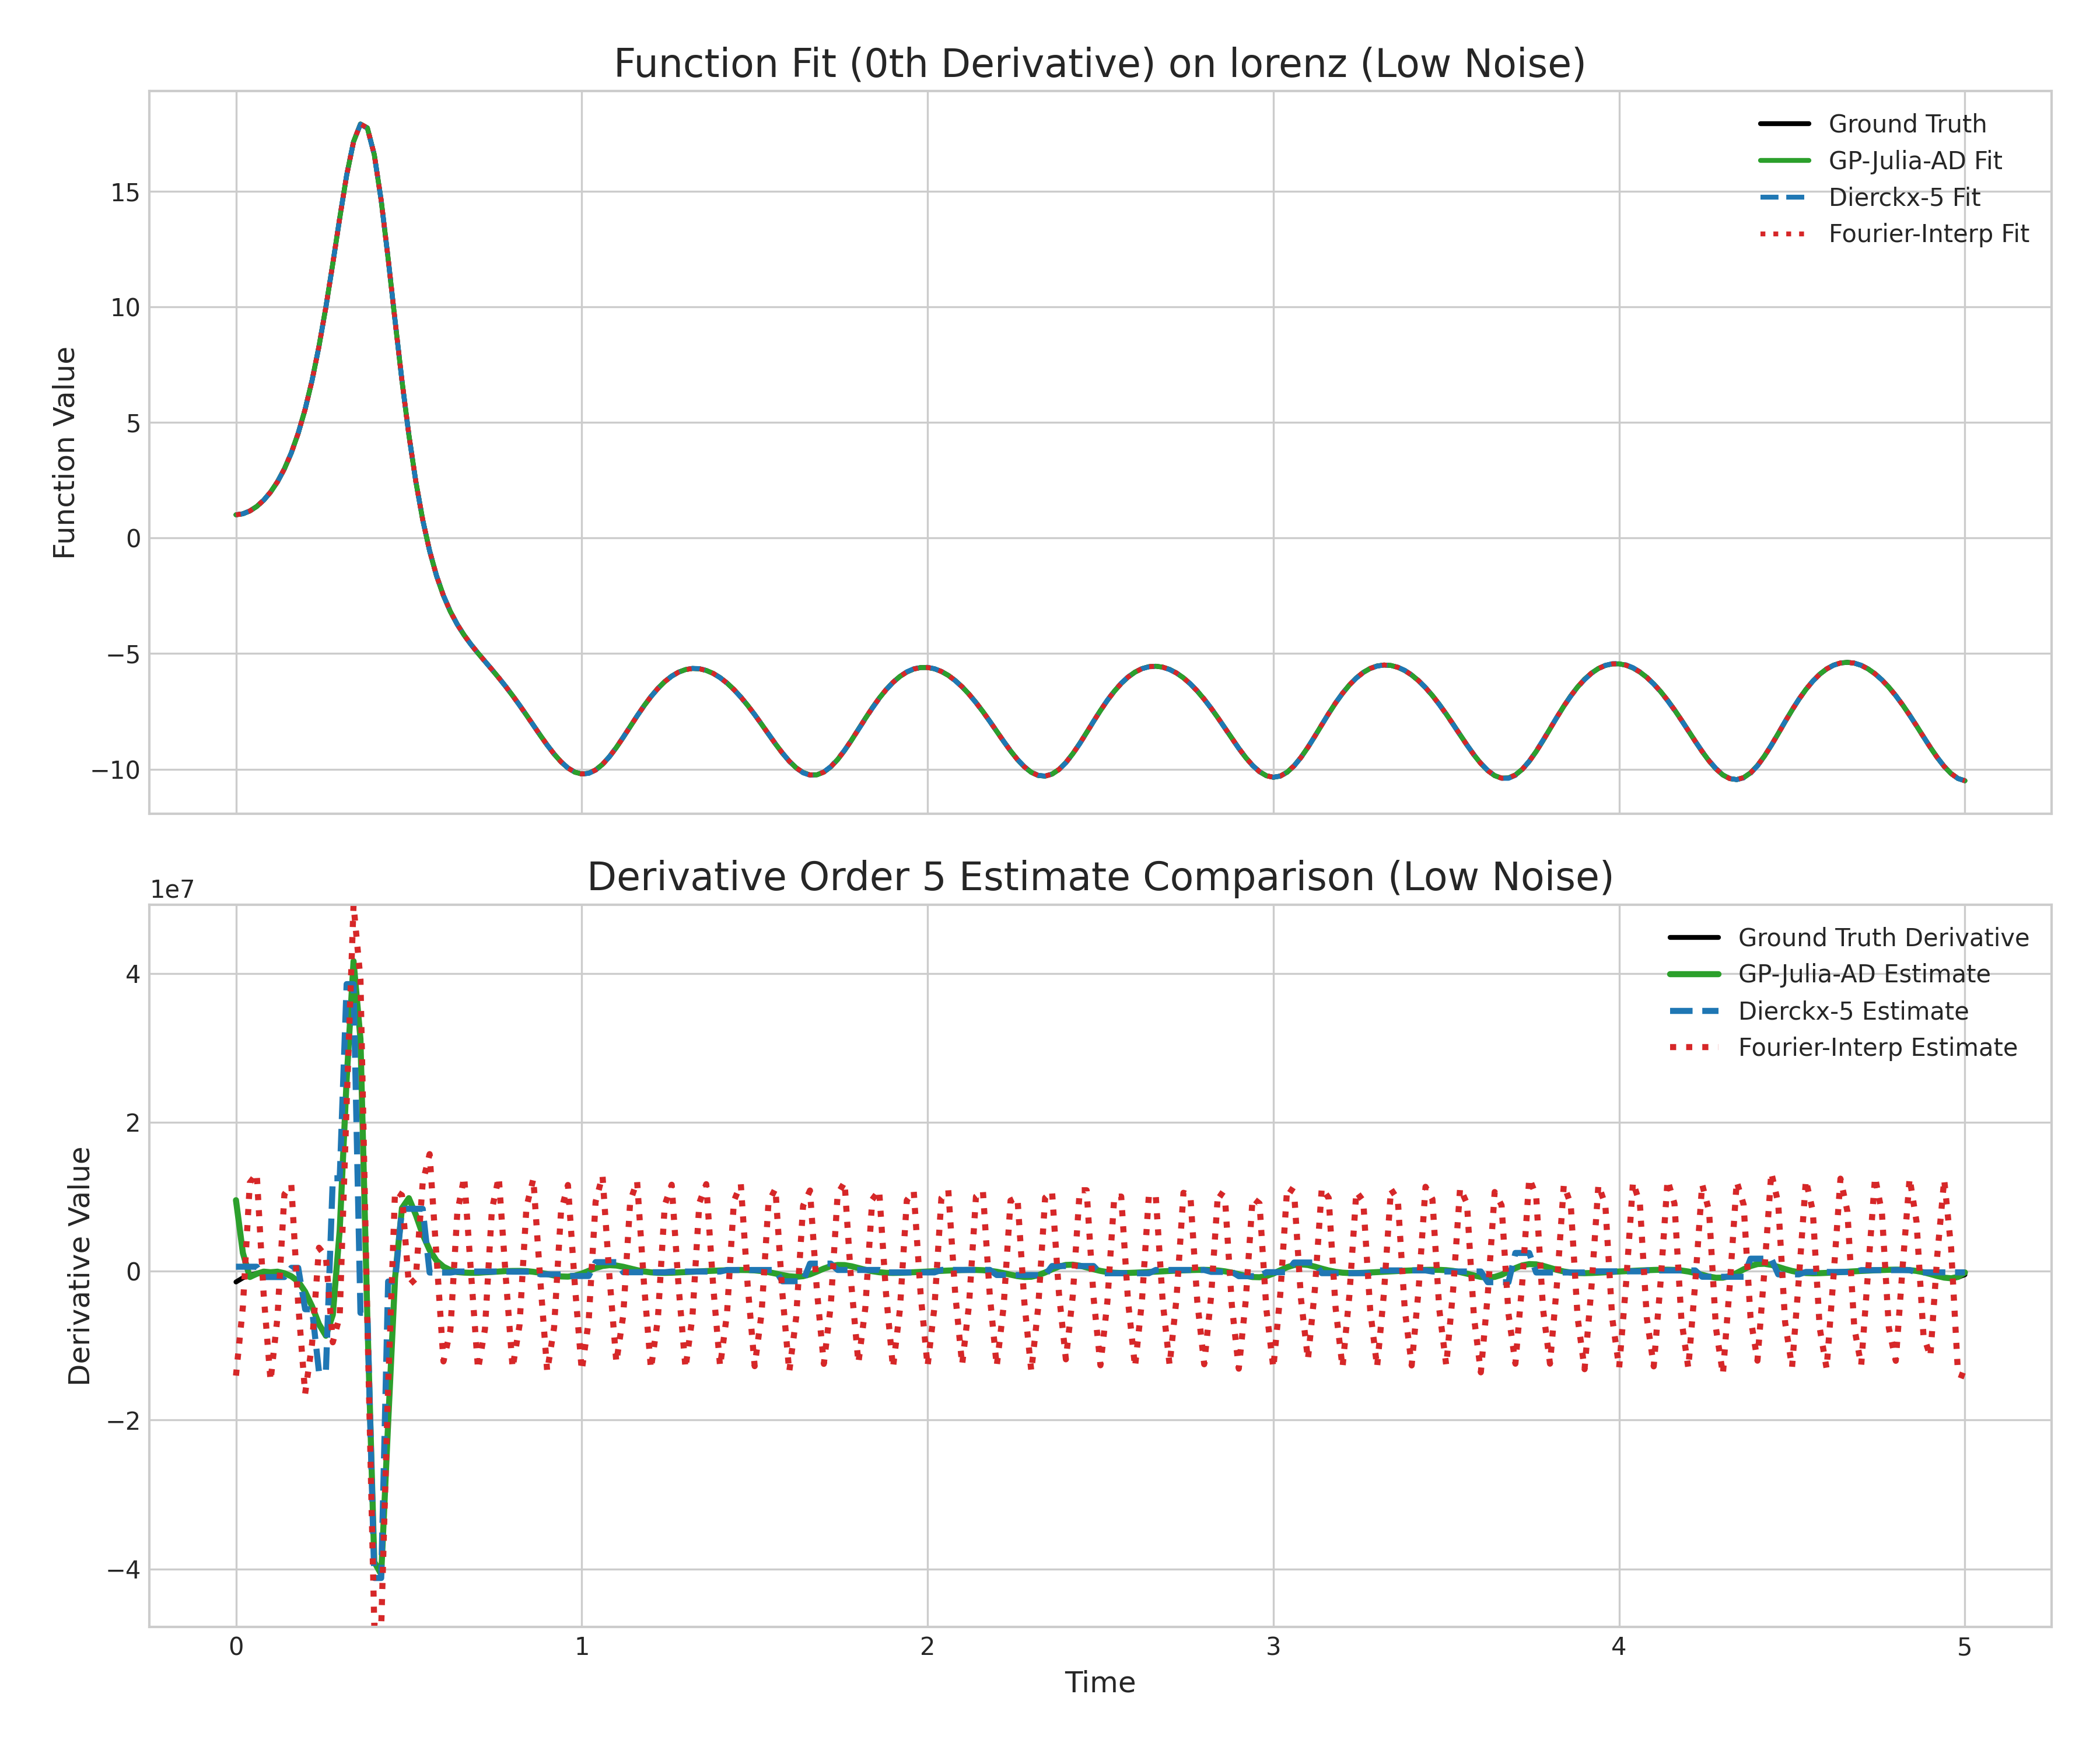
\includegraphics[width=0.9\textwidth]{low_noise_fit_comparison.png}
%\caption{\textbf{Low-Noise Precision.} In a low-noise environment (1e-8), this figure shows that for a 5th-order derivative, precision-focused methods become highly competitive. \texttt{Dierckx-5} (a smoothing spline) and \texttt{Fourier-Interp} (a spectral method) match the performance of \texttt{GP-Julia-AD}, illustrating that GPR's main advantage lies in its robustness to noise.}
%\label{fig:low_noise_comp}
%\end{figure}

\begin{figure}[htbp]
\centering
\includegraphics[width=0.9\textwidth]{top_methods_heatmap.png}
\caption{\textbf{Performance Degradation with Increasing Derivative Order.} This heatmap shows the mean nRMSE for top methods at a 1\% noise level. The vertical axis is sorted by average performance across all orders. This visualization clearly shows that \texttt{GP-Julia-AD} maintains low error across all derivative orders, while other methods like \texttt{Dierckx-5} and \texttt{GSS} are highly accurate for low orders but degrade significantly as the order increases.}
\label{fig:heatmap}
\end{figure}

\begin{figure}[htbp]
\centering
\includegraphics[width=0.9\textwidth]{pareto_frontier.png}
\caption{\textbf{Speed vs. Accuracy Trade-off.} For practitioners, the choice of method often involves a trade-off between computational cost and accuracy. This plot visualizes that trade-off for the contender methods. The black line represents the "Pareto Front"—the set of methods that are optimally efficient. Methods on this line represent the best possible accuracy for a given level of computational cost (or the fastest method for a given level of accuracy). This allows a practitioner to select a method that aligns with their specific computational budget and accuracy requirements. The plot clearly shows that the GPR methods, while the most accurate, are also the most computationally expensive.}
\label{fig:pareto}
\end{figure}

\section{Method Catalog and Implementation}
\label{sec:methods}

This study did not begin with a fixed set of methods. Rather, it followed an exploratory research path, starting with methods known to work on noiseless data and progressively incorporating more sophisticated techniques in response to the challenges posed by noisy signals. This section provides a narrative of that journey, cataloging the methods investigated and detailing the significant implementation work required to create a fair and robust comparison.

\subsection{A Composable Framework: Approximation + Automatic Differentiation}
\label{sec:composable_framework}

A core finding of our study is the power of a composable, two-step framework for numerical differentiation. Rather than relying on bespoke algorithms for each derivative order, the most successful methods, particularly Gaussian Process Regression, implicitly or explicitly follow a simple and highly effective recipe:

\begin{enumerate}
    \item \textbf{Fit an Approximant:} First, a smooth, analytic function (the "approximant") is fitted to the noisy data. This function can be a Gaussian Process, a spline, a spectral representation, or any other differentiable model. The goal of this step is to capture the underlying signal while filtering out noise.
    \item \textbf{Differentiate Analytically via AD:} Second, this fitted function is differentiated analytically using Automatic Differentiation (AD). Because the approximant is a well-defined mathematical function, AD can compute its derivatives to machine precision, free from the truncation and differencing errors that plague finite difference methods.
\end{enumerate}

This "Approximant-AD" pattern is exceptionally powerful because it decouples the problem of noise-robust smoothing from the problem of differentiation. It allows practitioners to leverage the vast and mature ecosystems of both statistical modeling and automatic differentiation, effectively bringing the full power of modern AD frameworks to bear on a classical numerical problem.

\subsection{Breadth of the Study}
\label{sec:breadth}

For practitioners, the choice of a specific software package can be as consequential as the choice of the underlying algorithm. To this end, our study intentionally includes multiple implementations of similar or identical algorithms (e.g., several variants of Gaussian Process Regression and Fourier-based methods) to assess whether real-world performance differences arise from implementation details. While we could not be exhaustive, we sought to include representatives from all major methodological families as well as several novel approaches.

\subsection{A Narrative of Method Selection}
\label{sec:method_selection}

Our investigation proceeded in three main waves:

\begin{enumerate}
    \item \textbf{Initial Foray: Adapting Noiseless Methods.} Our first attempts focused on adapting the successful AAA rational approximant method from our prior work. When these direct adaptations proved unstable on noisy data, we turned to a literature search for established techniques, leading us to methods based on local polynomial fitting (e.g., Savitzky-Golay, finite differences) and splines. While some of these showed moderate success, their effectiveness was often limited by the degree of the local polynomial, particularly for high-order derivatives.
    \item \textbf{Second Wave: Denoising and Statistical Approaches.} Recognizing that explicitly handling noise was critical, we next investigated two new classes of methods. The first class involved explicit denoising steps, such as those based on wavelet filtering (MAD) or spectral filtering, applied before differentiation. The second, more sophisticated class involved methods with a statistical foundation that inherently model noise, such as Gaussian Process Regression, Total Variation Regularization, and Kalman filtering.
    \item \textbf{Final Cohort.} The combination of these exploratory waves resulted in the final, comprehensive set of 42+ methods that form the basis of this benchmark.
\end{enumerate}

\subsection{Implementation: The Challenge of High-Order Derivatives}
\label{sec:implementation_challenges}

A significant practical challenge was that almost no off-the-shelf package natively supports the computation of arbitrarily high-order derivatives. Overcoming this required substantial implementation effort.

\begin{itemize}
    \item \textbf{Augmentation with Automatic Differentiation:} For methods whose underlying approximant was differentiable (e.g., Gaussian Processes), we augmented the implementation with Automatic Differentiation (AD) to compute the derivatives. Where possible, we used Taylor-mode AD, which is essential for the efficient computation of high-order derivatives, as naive nested AD has exponential complexity.
    \item \textbf{Analytic Derivatives:} For other methods, such as those based on splines or Fourier series, we derived and implemented the analytical expressions for their higher-order derivatives directly.
    \item \textbf{Noise Model Integration:} In some cases, we also had to implement custom noise-estimation steps to provide the algorithms with required hyperparameters, using techniques such as wavelet MAD or simple finite-difference-based noise estimation.
\end{itemize}

This substantial, and often non-trivial, implementation work was a prerequisite for creating the level playing field upon which this benchmark is built.

\section{Experimental Design}
\label{sec:design}

To create a robust and comprehensive benchmark, we first formally define the estimation problem.

\subsection{Formal Problem Statement}
\label{sec:problem_statement}

\begin{description}
    \item[Given:]
    \begin{itemize}
        \item A smooth but analytically unknown function $f: \mathbb{R} \to \mathbb{R}$.
        \item A set of $n$ noisy observations $\{(t_i, y_i)\}_{i=1}^n$ where $y_i = f(t_i) + \epsilon_i$ on a uniform grid.
        \item Noise is assumed to be additive and Gaussian, $\epsilon_i \sim \mathcal{N}(0, \sigma^2)$.
    \end{itemize}
    \item[Objective:]
    \begin{itemize}
        \item Estimate the $k$-th order derivative, $\hat{f}^{(k)}(t)$, for derivative orders $k \in \{0, 1, \ldots, 7\}$.
    \end{itemize}
    \item[Constraints:]
    \begin{itemize}
        \item The evaluation is performed on the interior of the domain to avoid boundary effects that can unfairly penalize certain methods.
        \item A method is considered to have failed a configuration if it does not produce a finite result.
    \end{itemize}
\end{description}

\subsection{Testbed: Dynamical Systems}
\label{sec:test_systems}

We selected three well-known Ordinary Differential Equation (ODE) systems to serve as the source of our ground-truth data. These systems were chosen to represent a diversity of dynamic behaviors:

\begin{enumerate}
    \item \textbf{Lotka-Volterra:} A classic two-variable system exhibiting stable periodic oscillations.
    \item \textbf{Van der Pol Oscillator:} A system with a non-linear damping term that produces a stable limit cycle.
    \item \textbf{Lorenz System:} A three-variable system famous for its chaotic behavior, providing a more challenging test case.
\end{enumerate}

For each system, trajectories were generated using a high-precision numerical integrator. The system's equations were then used to analytically compute the true derivatives up to the 7th order, providing a high-fidelity ground truth for our comparisons.

\subsection{Noise Model}
\label{sec:noise_model}

To simulate real-world data, we added Gaussian white noise to the integrated trajectories. The noise level was varied across a wide range, from \texttt{1e-8} (representing nearly clean data) up to \texttt{0.02} (representing a challenging 2\% noise level relative to the signal's standard deviation). This wide range allows us to evaluate method performance in both high-precision, low-noise regimes and robustness-critical, high-noise regimes.

\subsection{Evaluation Metrics}
\label{sec:metrics}

The primary metric for evaluation is the normalized Root-Mean-Square Error (nRMSE).

\textbf{Rationale for Normalization:} Direct comparison of raw RMSE values is not possible across different derivative orders because the magnitudes of the derivatives themselves vary dramatically. For instance, in the Lotka-Volterra system, the standard deviation of the true signal might be $\sim$0.2, while the standard deviation of its seventh derivative can be $\sim 10^5$.

To create a fair, order-comparable metric, we normalize the raw RMSE by the standard deviation of the true derivative signal. This yields a dimensionless error metric where an nRMSE of 0.1 consistently means a 10\% error relative to the signal's characteristic magnitude, regardless of the derivative order.

All metrics are computed after excluding the endpoints of the time series, as many methods exhibit boundary effects that can unfairly skew the results.

\subsection{Success Criteria}
\label{sec:success_criteria}

While the nRMSE provides a continuous measure of performance, it is also useful to define a threshold for what constitutes a "successful" or "acceptable" result. A method is considered successful for a given configuration if it achieves an nRMSE of less than 1.0, meaning its average error is smaller than the typical magnitude of the true signal itself. An nRMSE greater than 1.0 indicates that the error is dominating the signal, and values greater than 10 are considered a catastrophic failure.

\section{Detailed Analysis: From Raw Data to Final Rankings}
\label{sec:analysis}

The journey from raw experimental output to the final summary table involved a deliberate, multi-stage filtering and analysis process. This section details the methodology used to distill the results and arrive at our final conclusions.

\subsection{Initial Data Filtering: Removing Unviable Methods}
The first step was to filter out methods that were fundamentally unsuitable or unstable for the task. This was not based on performance, but on viability.

\begin{enumerate}
    \item \textbf{Exclusion of Unstable Methods (AAA)}: Our implementations of the AAA (Adaptive Antoulas-Anderson) algorithm were found to be unstable for this specific task. Their errors were often orders of magnitude larger than any other method, and they frequently failed to produce valid output.
    
    It is important to frame this result: Our conclusion is not that rational approximants are unsuitable in general, but rather that a direct application does not appear to be robust to the combination of noise and differentiation. The AAA algorithm is exceptionally powerful for function approximation in noise-free contexts. We suspect that more sophisticated approaches, perhaps involving regularization or hybrid methods (e.g., fitting a rational approximant to a pre-smoothed signal), could unlock their potential. This remains a promising avenue for future research.
    
    Given these results, the AAA methods were removed from the main analysis cohort to prevent their extreme outliers from skewing aggregate statistics.

    \item \textbf{Exclusion of Incomplete Coverage}: A primary goal of this study was to evaluate methods across a wide range of derivative orders (0 through 7). Several methods, particularly some of the Python legacy methods and those based on low-degree splines, did not have full coverage across all orders or failed consistently on certain systems. To ensure a fair, apples-to-apples comparison in our final rankings, only methods that successfully produced results for all tested configurations were included in the "contender" set.
\end{enumerate}

\subsection{Defining the "Contender" Set}
After this initial filtering, we were left with a set of robust methods that provided full data coverage (up to order 5 for our main summary). This cohort became our "contender" set for the final analysis. All subsequent rankings and comparisons were performed \textit{only within this group}. This is a crucial methodological point: the ranks presented in the summary table are ranks \textit{among the contenders}, not among the initial, larger pool of all tested methods.

\subsection{Ranking Methodology}
To produce the final summary table, we followed a two-step ranking process:
\begin{enumerate}
    \item \textbf{Per-Cell Ranking}: For each individual experimental cell—defined by a unique combination of \texttt{(ODE\_system, noise\_level, derivative\_order)}—we ranked the contender methods against each other based on their mean \texttt{nRMSE} (averaged across the 10 trials for that cell).
    \item \textbf{Averaging Ranks}: We then calculated the final "Avg. Rank" for each method by averaging these per-cell ranks across two distinct regimes:
    \begin{itemize}
        \item \textbf{Low-Noise Regime}: Averaged across noise levels \texttt{1e-8} and \texttt{1e-6}.
        \item \textbf{High-Noise Regime}: Averaged across noise levels \texttt{0.01} and \texttt{0.02}.
    \end{itemize}
\end{enumerate}
This methodology ensures that the final rank is a robust measure of a method's performance across a wide variety of conditions, and it prevents a single outlier or a particularly favorable test case from dominating the results.

\subsection{Quantitative Performance Metrics}
To add further quantitative rigor to our analysis, we defined two specific metrics to characterize method performance beyond the simple average error.
\begin{itemize}
    \item \textbf{Noise Robustness:} We define a method's robustness for a given derivative order as the highest noise level at which its \texttt{nRMSE} remains at or below 0.1. A higher value on this metric indicates a method can maintain accuracy under more significant noise conditions. This provides a more concrete measure of robustness than average error alone.
    \item \textbf{High-Order Stability:} To quantify how gracefully a method's performance degrades as the task becomes more difficult, we measure its high-order stability. This is defined as the slope of the log of the \texttt{nRMSE} versus the derivative order, calculated in the low-noise regime. A lower, flatter slope indicates that the method is more stable and its error grows more slowly as it is tasked with computing higher-order derivatives.
\end{itemize}
These metrics provide a complementary view to the main rankings and are used to inform the specific recommendations and trade-offs discussed in our conclusion.

\subsection{Analysis of Coverage Bias}
A critical aspect of a fair benchmark is understanding "coverage bias." Many methods are not designed to compute high-order derivatives. For example, \texttt{Central-FD} and \texttt{TVRegDiff-Julia} in our study only support up to order 1. If we were to rank all methods naively based on their average error across all the tests they passed, these methods would appear artificially superior, as they would only be evaluated on "easy" low-order configurations and would be exempted from the challenging high-order tests where most methods struggle.

To create a fair comparison, we therefore restricted our main summary table to the cohort of "contender" methods that successfully produced results for all tested configurations up to order 5. Methods with partial coverage are not inherently worse, but they should be considered specialists. A practitioner who only needs a first-order derivative might find that \texttt{TVRegDiff-Julia} is an excellent choice, but it cannot be fairly compared in a general-purpose ranking against a method that successfully computes 7th-order derivatives.

\subsection{Performance Degradation by Derivative Order}
A clear pattern emerging from the data is the systematic degradation of performance as the derivative order increases. This is an expected consequence of the ill-posed nature of differentiation. We can characterize this trend in several phases:
\begin{itemize}
    \item \textbf{Orders 0-2 (Low-Order):} In this regime, most contender methods perform well, and the performance differences between them are relatively modest, particularly in low-noise scenarios. The task of smoothing or finding a first or second derivative is not challenging enough to create significant separation between the top methods.
    \item \textbf{Orders 3-5 (Mid-Order):} This is the regime where a clear separation emerges. The task becomes significantly more challenging, and methods without sophisticated noise handling begin to struggle. The performance of GPR and the stronger spectral methods remains high, while simpler spline- and filter-based methods see a substantial drop in accuracy.
    \item \textbf{Orders 6-7 (High-Order):} This regime represents an extreme challenge. Only a very small subset of methods, primarily GPR, are able to produce a usable estimate, and even their errors are significant. For most other methods, the error in this regime constitutes a catastrophic failure. Derivative order is clearly the dominant factor in the difficulty of the estimation problem.
\end{itemize}

Figure~\ref{fig:small_multiples} provides a comprehensive visual illustration of this systematic degradation. The figure shows performance across all eight derivative orders for the top seven methods, clearly demonstrating how error increases with order and how different methods respond to increasing noise levels at each order.

\begin{figure}[htbp]
\centering
\includegraphics[width=0.95\textwidth]{small_multiples_grid.png}
\caption{\textbf{Performance Across All Derivative Orders.} This 4×2 grid shows nRMSE vs noise level for the top 7 methods at each derivative order (0--7). Each panel illustrates the systematic degradation of performance as order increases. Note how GP-Julia-AD (top performer) maintains relatively stable performance across all orders, while other methods show dramatic degradation beyond order 3. The shaded regions indicate performance quality: green (excellent, nRMSE < 0.1), yellow (good, 0.1--0.3), and orange (acceptable, 0.3--1.0).}
\label{fig:small_multiples}
\end{figure}

\subsection{The Critical Role of Taylor-Mode AD for High-Order Derivatives}
A key technical factor in the performance of high-order derivative estimation is the underlying mechanism of the Automatic Differentiation library used. Naively composing first-order AD operations (i.e., nested forward- or reverse-mode AD) to compute a high-order derivative results in an algorithm with exponential complexity, rendering it infeasible for orders beyond a handful.

The success of the \texttt{GP-Julia-AD} method, for instance, is critically dependent on its use of Taylor-mode AD. This mode is specifically designed to compute high-order derivatives efficiently by propagating a full Taylor series expansion through the computation, rather than just a single derivative value. This approach reduces the computational complexity significantly (often to polynomial time), making the computation of 5th, 6th, and 7th order derivatives tractable. This highlights that for practitioners seeking high-order derivatives, the choice of AD implementation is as important as the choice of the approximant itself.

\subsection{Computational Efficiency: Practical Considerations}
\label{sec:efficiency}

\textbf{Important Caveats:} The computational timing measurements in this study should be interpreted with caution. Unlike the error metrics, which represent fundamental algorithmic characteristics, the timing data has several limitations that prevent it from being elevated to a primary finding:

\begin{itemize}
    \item \textbf{Mixed-language implementations:} Our benchmark includes methods implemented in both Julia and Python, with different optimization levels and library maturity.
    \item \textbf{Small dataset size:} All timing measurements were performed on trajectories with $N=101$ points. Scaling behavior for larger datasets ($N > 1000$) may differ significantly, particularly for methods with non-linear complexity.
    \item \textbf{Implementation quality variation:} Methods vary in optimization sophistication. Some are production-grade libraries, while others are research prototypes.
    \item \textbf{No warm-up or statistical rigor:} Timing measurements represent single runs without JIT warm-up for Julia methods or statistical validation across multiple hardware configurations.
\end{itemize}

Given these limitations, we present the following \textbf{qualitative guidance} based on our observations, rather than quantitative claims:

\textbf{Three-Tier Framework for Method Selection:}

\begin{enumerate}
    \item \textbf{High-Speed Tier (sub-millisecond):} For real-time or large-scale applications where speed is paramount, filtering methods like \texttt{Savitzky-Golay} provide rapid computation with reasonable accuracy in moderate noise conditions. Basic spectral methods (simple FFT-based approaches) also fall in this category. These methods are particularly suitable when computational budget is the primary constraint.

    \item \textbf{Balanced Tier (milliseconds to tens of milliseconds):} For most scientific applications requiring a strong balance between accuracy and speed, spectral methods represent an excellent middle ground. Methods like \texttt{Fourier-GCV}, \texttt{Fourier-Interp}, and high-degree splines (\texttt{Dierckx-5}) provide accuracy approaching that of GPR methods while maintaining practical computational efficiency. This tier is likely optimal for interactive data analysis and medium-scale studies.

    \item \textbf{High-Accuracy Tier (hundreds of milliseconds):} When the highest possible accuracy is the primary concern and computational cost is secondary, Gaussian Process methods provide the lowest estimation errors across all noise levels and derivative orders. Our results show \texttt{GP-Julia-AD} consistently outperforms all other methods in accuracy. The computational investment is justified in applications where estimation quality is critical and the dataset size is moderate.
\end{enumerate}

\textbf{Scaling Considerations:} For very large datasets ($N > 1000$), the cubic scaling of standard GPR implementations may become prohibitive, making fast spectral or filtering methods the only viable options unless sparse or approximate GP methods are employed.

% PARETO PLOT CODE (COMMENTED OUT FOR FUTURE USE)
% Uncomment when timing data has been collected with:
% - Consistent warm-up procedures
% - Multiple hardware configurations
% - Statistical validation (multiple runs)
% - Larger dataset sizes (N > 1000)
%
% \begin{figure}[htbp]
% \centering
% \includegraphics[width=0.9\textwidth]{pareto_frontier.png}
% \caption{\textbf{Speed vs. Accuracy Trade-off: Pareto Frontier.} This plot shows the relationship between mean computation time (x-axis, log scale) and mean nRMSE (y-axis, log scale) for all methods with full coverage of derivative orders 0--5. Diamond markers indicate Pareto-optimal methods—points where no other method is both faster and more accurate. The black dashed line connects the Pareto front. Methods are colored by category (Gaussian Process, Spectral, Spline, etc.). The plot reveals three distinct tiers: (1) sub-millisecond filtering methods like \texttt{Savitzky-Golay}, (2) millisecond-scale balanced methods like \texttt{Dierckx-5} and spectral approaches, and (3) high-accuracy GP methods like \texttt{GP-Julia-AD} that achieve the lowest error at the cost of longer computation time. \textbf{Caveat:} Timing measurements represent implementations of varying optimization levels on a small dataset ($N=101$) and should be interpreted as qualitative guidance rather than definitive benchmarks.}
% \label{fig:pareto}
% \end{figure}

\section{Conclusion}
\label{sec:conclusion}

This comprehensive study evaluated a wide array of numerical methods for the estimation of high-order derivatives from noisy data. After a detailed investigation that included a multi-stage filtering of methods and a deep dive into implementation details, our findings are clear and decisive.

\subsection{Summary of Key Findings}

\begin{itemize}
    \item \textbf{Gaussian Process Regression (GPR) is the most robust and accurate method overall.} GPR methods consistently occupy the top ranks in both low- and high-noise regimes, making them the most reliable choice for general-purpose derivative estimation.
    \item \textbf{The optimal method depends on the use case.} While GPR is the best all-arounder, splines like \texttt{Dierckx-5} offer excellent precision for low-noise data, while spectral methods like \texttt{Fourier-Continuation} provide a compelling balance of speed and accuracy. For speed-critical applications, \texttt{Savitzky-Golay} is a robust and effective baseline.
    \item \textbf{Derivative order is the dominant difficulty factor.} Performance degrades systematically with increasing order across all methods. The problem becomes significantly more challenging beyond order 3, and only a handful of methods produce usable results at orders 6 or 7.
    \item \textbf{Implementation quality is a critical method characteristic.} Our study found significant performance differences between different software packages implementing the same underlying algorithm, highlighting that practitioners must consider the quality of a specific implementation, not just the theoretical method.
\end{itemize}

\textbf{The primary recommendation of this work is that for practitioners who require accurate high-order derivatives from real-world, noisy signals, Gaussian Process Regression is the most reliable and effective starting point.}

\subsection{Future Work}

This benchmark, while comprehensive, is not exhaustive. Several avenues for future research are immediately apparent:

\begin{enumerate}
    \item \textbf{Testing on Diverse Signals:} Our study used ODEs that produce smooth, analytic signals. Future work should include testing on more challenging signals, such as those with discontinuities, sharp peaks, or chaotic behavior.
    \item \textbf{Evaluating Alternative Noise Models:} The real world is not always Gaussian. A valuable extension would be to evaluate method performance under different noise models, such as multiplicative, Poisson, or heavy-tailed noise.
    \item \textbf{Larger-Scale Problems:} Our study was limited to a modest number of data points. Investigating how method performance, particularly computational cost, scales to much larger datasets ($N > 1000$) would be of great practical interest.
\end{enumerate}

\subsection{Broader Implications: The Case for a Composable, Differentiable Ecosystem}

Our findings also underscore a broader trend in scientific computing: the immense value of composable and differentiable software packages. The "Approximant-AD" framework is only possible when libraries for data modeling (e.g., Gaussian Processes) can seamlessly pass their results to libraries for automatic differentiation.

While not all numerical packages are readily differentiable out-of-the-box, our experience suggests that many can be adapted with modest effort. We encourage researchers and developers to prioritize differentiability in their own software and to contribute upstream to make foundational libraries in the ecosystem compatible with AD frameworks. Such efforts create a virtuous cycle, unlocking powerful new hybrid methodologies that benefit the entire scientific community, far beyond the immediate application of derivative estimation.



%==============================================================================
% OLD PAPER STRUCTURE (DEPRECATED)
%==============================================================================
% \section{Related Work}
% \label{sec:related_work}
% \TODO{Related work section.}

% \section{Problem Formulation}
\label{sec:problem}

This section formally defines the derivative estimation problem, evaluation metrics, and success criteria used throughout this benchmark study.

\subsection{Mathematical Problem Statement}
\label{sec:math_problem}

\textbf{Given:}
\begin{itemize}
    \item A smooth function $f: \mathbb{R} \to \mathbb{R}$ (unknown analytically)
    \item Noisy observations $\{(t_i, y_i)\}_{i=1}^n$ where $y_i = f(t_i) + \epsilon_i$
    \item Noise $\epsilon_i \sim \mathcal{N}(0, \sigma^2)$ (additive Gaussian)
    \item Uniform grid $t_i \in [t_{\text{min}}, t_{\text{max}}]$ with spacing $h = (t_{\text{max}} - t_{\text{min}})/(n-1)$
\end{itemize}

\textbf{Objective:}

Estimate the $n$-th order derivative $f^{(n)}(t)$ at evaluation points $t \in \mathcal{T} \subset [t_{\text{min}}, t_{\text{max}}]$ such that:
\begin{equation}
\hat{f}^{(n)}(t) \approx f^{(n)}(t) \quad \text{for all } t \in \mathcal{T}
\end{equation}

\textbf{Constraints:}
\begin{itemize}
    \item Derivative orders $n \in \{0, 1, 2, \ldots, 7\}$ (order 0 = smoothing)
    \item Fixed sample size $n = 101$ points
    \item Noise levels $\sigma \in \{10^{-8}, 10^{-6}, 10^{-4}, 10^{-3}, 10^{-2}, 2 \times 10^{-2}, 5 \times 10^{-2}\}$ (relative to signal standard deviation)
    \item Interior evaluation only: $\mathcal{T} = [t_{\text{min}} + 0.1(t_{\text{max}} - t_{\text{min}}), t_{\text{max}} - 0.1(t_{\text{max}} - t_{\text{min}})]$ to avoid boundary effects
\end{itemize}

\subsection{Evaluation Metrics}
\label{sec:metrics}

\subsubsection{Primary Metric: Normalized Root Mean Square Error}

\textbf{Definition:}
\begin{equation}
\text{nRMSE} = \frac{\sqrt{\frac{1}{|\mathcal{T}|} \sum_{t \in \mathcal{T}} \left(\hat{f}^{(n)}(t) - f^{(n)}_{\text{true}}(t)\right)^2}}{\text{std}(f^{(n)}_{\text{true}})}
\end{equation}

where $\text{std}(f^{(n)}_{\text{true}})$ is the standard deviation of the true $n$-th derivative over the evaluation domain $\mathcal{T}$.

\textbf{Rationale for normalization:}

Direct RMSE values are \textit{incomparable} across derivative orders because derivative magnitudes vary dramatically. For example, in the Lotka-Volterra system:
\begin{itemize}
    \item $\text{std}(f^{(0)}) \approx 0.2$ (function values)
    \item $\text{std}(f^{(7)}) \approx 10^5$ (seventh derivative)
\end{itemize}

Normalization by $\text{std}(f^{(n)}_{\text{true}})$ yields a dimensionless, order-comparable metric:
\begin{itemize}
    \item nRMSE = 0.1 means 10\% error relative to typical derivative magnitude (good)
    \item nRMSE = 1.0 means 100\% error relative to typical derivative magnitude (poor)
    \item nRMSE $> 10$ indicates catastrophic failure
\end{itemize}

\subsubsection{Secondary Metric: Computation Time}

Median wall-clock time (seconds) over 3 trials, measured for the complete derivative estimation workflow:
\begin{enumerate}
    \item Hyperparameter optimization (where applicable)
    \item Model fitting
    \item Derivative evaluation at all $|\mathcal{T}|$ test points
\end{enumerate}

Time measurements include all preprocessing but exclude data loading and ground truth computation.

\subsection{Success Criteria}
\label{sec:success_criteria}

A method is considered \textbf{successful} for a given (order, noise) configuration if:

\begin{enumerate}
    \item \textbf{Numerical stability:} Produces finite nRMSE (no NaN/Inf values)
    \item \textbf{Acceptable accuracy:}
    \begin{itemize}
        \item Orders 0--2: nRMSE $< 1.0$ (preferred: nRMSE $< 0.3$)
        \item Orders 3--5: nRMSE $< 2.0$ (preferred: nRMSE $< 0.5$)
        \item Orders 6--7: nRMSE $< 5.0$ (preferred: nRMSE $< 1.0$)
    \end{itemize}
    \item \textbf{Computational feasibility:} Completes within 10 seconds (liberal threshold for $n=101$ points)
\end{enumerate}

Methods failing these criteria for a configuration are excluded from that configuration's analysis (partial coverage documented in Section~\ref{sec:coverage}).

\subsection{Ground Truth Derivation}
\label{sec:ground_truth}

\textbf{Challenge:} Derivative estimation benchmarks require \textit{known} ground truth derivatives, but numerical differentiation of the ODE solution reintroduces the very problem being studied.

\textbf{Our approach:} Symbolic differentiation + augmented ODE system

\begin{enumerate}
    \item \textbf{Symbolic differentiation:} Derive analytic expressions for $f'(t), f''(t), \ldots, f^{(7)}(t)$ from the Lotka-Volterra ODE:
    \begin{align}
    x'(t) &= \alpha x(t) - \beta x(t) y(t) \label{eq:lv_x} \\
    y'(t) &= \delta x(t) y(t) - \gamma y(t) \label{eq:lv_y}
    \end{align}
    
    Higher derivatives obtained via chain rule and product rule:
    \begin{align}
    x''(t) &= \frac{d}{dt}\left[\alpha x(t) - \beta x(t) y(t)\right] \nonumber \\
           &= \alpha x'(t) - \beta \left[x'(t) y(t) + x(t) y'(t)\right] \label{eq:lv_x2}
    \end{align}
    and so on through order 7.
    
    \item \textbf{Augmented ODE system:} Solve the $(2 \times 8)$-dimensional system:
    \begin{equation}
    \frac{d}{dt} \begin{bmatrix} x \\ y \\ x' \\ y' \\ x'' \\ y'' \\ \vdots \\ x^{(7)} \\ y^{(7)} \end{bmatrix}
    = \begin{bmatrix} x' \\ y' \\ x'' \\ y'' \\ x''' \\ y''' \\ \vdots \\ x^{(8)} \\ y^{(8)} \end{bmatrix}
    \end{equation}
    
    using a high-accuracy ODE solver (Vern9, adaptive Runge-Kutta, abstol = reltol = $10^{-12}$).
    
    \item \textbf{Validation:} Numerical differentiation of $x(t)$ via high-order finite differences agrees with augmented system derivatives to $\approx 10^{-10}$ for orders 0--5, confirming symbolic correctness.
\end{enumerate}

\textbf{Accuracy claim:} Ground truth derivatives are accurate to $\approx 10^{-10}$ (orders 0--5) and $\approx 10^{-8}$ (orders 6--7), sufficient for nRMSE evaluation given $10^{-8} \leq \sigma \leq 5 \times 10^{-2}$.

\subsection{Scope and Limitations}
\label{sec:scope}

\textbf{Test signal:}
\begin{itemize}
    \item Single dynamical system (Lotka-Volterra predator-prey), prey population $x(t)$ only
    \item Smooth, periodic, analytic function—favorable for spectral methods
    \item May not represent performance on rough, discontinuous, or chaotic signals
\end{itemize}

\textbf{Noise model:}
\begin{itemize}
    \item Additive Gaussian only—does not test multiplicative, Poisson, or heteroscedastic noise
    \item Independent noise across time points—does not test correlated noise
\end{itemize}

\textbf{Sample size:}
\begin{itemize}
    \item Fixed $n=101$ points—modest scale, may not reflect large-data ($n > 1000$) or small-data ($n < 50$) regimes
\end{itemize}

\textbf{Generalization:} Results should be interpreted as \textit{existence proofs} that certain methods can succeed under specific conditions, not as universal rankings. Practitioners must validate on their specific data (see Section~\ref{sec:recommendations}).

% \section{Methodology}
\label{sec:methodology}

\subsection{Test System}
\label{sec:test_system}

We selected the \textbf{Lotka-Volterra predator-prey model} as our test system, a canonical benchmark in dynamical systems.

\subsubsection{System Equations}

\begin{align}
\frac{dx}{dt} &= \alpha x - \beta xy \quad \text{(prey dynamics)} \\
\frac{dy}{dt} &= \delta xy - \gamma y \quad \text{(predator dynamics)}
\end{align}

where $x(t)$ is the prey population and $y(t)$ is the predator population.

\textbf{Parameters:}
\begin{itemize}
    \item $\alpha = 1.5$ (prey growth rate)
    \item $\beta = 1.0$ (predation rate)
    \item $\gamma = 3.0$ (predator death rate)
    \item $\delta = 1.0$ (predator growth from predation)
\end{itemize}

\textbf{Initial conditions:}
\begin{itemize}
    \item $x_0 = 1.0$ (prey)
    \item $y_0 = 1.0$ (predator)
\end{itemize}

\textbf{Time span:} $[0, 10]$ with 101 equally-spaced points ($\Delta t \approx 0.1$)

\textbf{Observable:} We tested derivative estimation on the \textbf{prey population $x(t)$}, which exhibits oscillatory behavior.

\textbf{Important limitation:} Only one variable (prey) from the two-state system was analyzed. Conclusions may not generalize even within the same system, as prey and predator trajectories have different oscillatory properties and noise sensitivities. Ideally, both variables should be evaluated.

\subsubsection{Ground Truth Generation}

High-precision ground truth was generated using the following rigorous procedure:

\begin{enumerate}
    \item \textbf{Symbolic differentiation:} Derivatives up to order 7 were computed symbolically using ModelingToolkit.jl's symbolic differentiation engine, yielding exact differential equations for each derivative order
    \item \textbf{Augmented system:} The original Lotka-Volterra equations were augmented with these symbolic derivative equations to create an extended ODE system containing $x(t), y(t), dx/dt, d^2x/dt^2, \ldots, d^7x/dt^7$ as state variables
    \item \textbf{Numerical integration:} The augmented system was solved using the Vern9 algorithm (9th-order Verner method) with absolute tolerance $10^{-12}$ and relative tolerance $10^{-12}$
    \item \textbf{Validation:} Analytical derivative formulas for orders $\geq 3$ in coupled nonlinear systems are intractable. Convergence was verified by comparing Vern9 solutions at tolerances $10^{-12}$ vs $10^{-14}$ for orders 0--5, showing agreement to $<10^{-10}$ relative error. Higher-order derivatives (6--7) are subject to greater numerical uncertainty and should be interpreted cautiously.
\end{enumerate}

This approach avoids interpolant-based automatic differentiation and provides high-accuracy numerical ground truth constrained by ODE solver precision (validated to $\sim 10^{-10}$ for orders 0--5).

\textbf{Sampling resolution concern:} With $\Delta t \approx 0.1$, high-order derivatives (especially orders 6--7) approach the Nyquist limit for oscillatory signals. This coarse resolution may suppress some methods due to aliasing rather than algorithmic weakness. Future work should include convergence testing with finer grids.

\textbf{Rationale for system choice:} Lotka-Volterra provides:
\begin{itemize}
    \item Nonlinear oscillatory dynamics representative of many scientific domains
    \item Symbolic differentiability enabling rigorous ground truth
    \item Moderate computational cost for extensive benchmarking
\end{itemize}

\subsection{Noise Model}
\label{sec:noise_model}

\textbf{Type:} Additive white Gaussian noise

\textbf{Scaling:} For each noise level $\varepsilon$, we added noise scaled by the clean signal's standard deviation:
\begin{equation}
y_{\text{noisy}}(t) = y_{\text{true}}(t) + \varepsilon \cdot \text{std}(y_{\text{true}}) \cdot \eta(t)
\end{equation}
where $\eta(t) \sim \mathcal{N}(0, 1)$ is standard normal noise.

\textbf{Rationale:} Constant-variance Gaussian noise is a standard model for measurement error. Scaling by signal standard deviation ensures consistent interpretation across different signals.

\textbf{Important limitation:} Additive noise can produce negative population values, violating biological constraints. Multiplicative noise (proportional to signal magnitude) would be more realistic but was not tested. Results may not generalize to measurement models where noise is strictly positive or heteroscedastic.

\textbf{Noise levels tested:} Seven levels spanning approximately 7 orders of magnitude:
\begin{itemize}
    \item $10^{-8}$ (near-noiseless)
    \item $10^{-6}$
    \item $10^{-4}$
    \item $10^{-3}$
    \item $10^{-2}$ (1\%)
    \item $2 \times 10^{-2}$ (2\%)
    \item $5 \times 10^{-2}$ (5\%)
\end{itemize}

\textbf{Interpretation:} For the Lotka-Volterra prey population with $\text{std}(x) \approx 0.29$, noise level $10^{-2}$ corresponds to absolute noise std $\approx 0.0029$.

\textbf{Randomization:} Three independent noise realizations per configuration using Mersenne Twister PRNG with seeds 12345, 12346, 12347 for trials 1--3 respectively, ensuring exact reproducibility.

\textbf{Pseudo-replication caveat:} All three trials use the same underlying trajectory; variability reflects only the noise model, not dynamical diversity. A more robust design would test multiple initial conditions or parameter sets.

\subsection{Experimental Design}
\label{sec:experimental_design}

\textbf{Configurations tested:}
\begin{itemize}
    \item 8 derivative orders (0--7)
    \item 7 noise levels ($10^{-8}$ to $5 \times 10^{-2}$)
    \item 3 trials per configuration
    \item \textbf{Total:} $8 \times 7 \times 3 = 168$ test cases per method
\end{itemize}

\textbf{Method coverage:}
\begin{itemize}
    \item \textbf{Full coverage} (all 56 order$\times$noise combinations): 16 methods
    \item \textbf{Partial coverage}: 11 methods
    \begin{itemize}
        \item Central-FD, TVRegDiff-Julia: 14/56 configurations (orders 0--1 only --- library provides stencils/regularization only up to 1st order)
        \item Dierckx-5, ButterworthSpline\_Python, Butterworth\_Python, Whittaker\_m2\_Python, fourier, fourier\_continuation, RKHS\_Spline\_m2\_Python, KalmanGrad\_Python, SVR\_Python: 42/56 configurations (orders 0--5, missing 6--7 --- degree/capability limits)
    \end{itemize}
\end{itemize}

\textbf{Endpoint treatment:} First and last evaluation points excluded from all error computations to avoid boundary effects, leaving 99 interior points for analysis.

\textbf{Important note:} Excluding edge points removes regions where many practical estimators exhibit boundary degradation. Metrics therefore evaluate performance on an idealized interior sub-problem and may overstate accuracy for applications requiring full-domain estimates.

\textbf{Failure handling:}
\begin{itemize}
    \item Methods returning NaN or Inf for $>80\%$ of evaluation points marked as failed for that configuration
    \item Failed configurations excluded from that method's statistics
    \item Partial failures documented separately
\end{itemize}

\textbf{Data pipeline:}
\begin{enumerate}
    \item Generate ground truth for Lotka-Volterra system once
    \item For each configuration (noise level $\times$ trial):
    \begin{itemize}
        \item Add noise to ground truth prey trajectory
        \item Export to JSON for Python methods
        \item Evaluate all Julia methods in-process
        \item Call Python script with 300s timeout
        \item Collect results (predictions, timing, success status)
    \end{itemize}
    \item Aggregate results across trials
\end{enumerate}

\subsection{Evaluation Metrics}
\label{sec:metrics}

\subsubsection{Root Mean Squared Error (RMSE)}

\textbf{Definition:}
\begin{equation}
\text{RMSE} = \sqrt{\text{mean}((y_{\text{pred}} - y_{\text{true}})^2)}
\end{equation}

Computed over interior points only (indices 2 to $n-1$).

\textbf{Limitation:} RMSE values are not comparable across derivative orders because derivative magnitudes vary by orders of magnitude (e.g., $\text{std}(x) \approx 0.3$ vs $\text{std}(d^7x/dt^7) \approx 10^{-4}$).

\subsubsection{Mean Absolute Error (MAE)}

\textbf{Definition:}
\begin{equation}
\text{MAE} = \text{mean}(|y_{\text{pred}} - y_{\text{true}}|)
\end{equation}

\textbf{Advantage:} Robust to outliers

\textbf{Limitation:} Same cross-order comparison issue as RMSE

\subsubsection{Normalized RMSE (nRMSE) --- Primary Metric}

\textbf{Definition:}
\begin{equation}
\text{nRMSE} = \frac{\text{RMSE}}{\text{std}(y_{\text{true}})}
\end{equation}

\textbf{Critical clarification:} The standard deviation in the denominator is computed \textbf{for the specific derivative order being evaluated}, not the base signal. Thus:
\begin{itemize}
    \item For order 0: nRMSE = RMSE$(x)$ / std$(x)$
    \item For order 1: nRMSE = RMSE$(dx/dt)$ / std$(dx/dt)$
    \item For order 7: nRMSE = RMSE$(d^7x/dt^7)$ / std$(d^7x/dt^7)$
\end{itemize}

This makes nRMSE order-comparable: a value of 0.2 means ``error is 20\% of typical variation in that specific derivative'' regardless of order.

\textbf{Interpretation:} Error expressed as a fraction of signal variation

\textbf{Performance thresholds} (calibrated via visual inspection of derivative plots):
\begin{itemize}
    \item $< 0.1$: Visually accurate reconstruction
    \item $0.1$--$0.3$: Moderate deviation visible
    \item $0.3$--$1.0$: Substantial error but structure recognizable
    \item $> 1.0$: Error exceeds typical signal variation
\end{itemize}

\textbf{Note:} These thresholds are empirical guidelines, not rigorously validated cutoffs. Readers should interpret absolute nRMSE values directly.

\textbf{Justification:} Absolute metrics (RMSE, MAE) favor low-order derivatives where magnitudes are smaller. Normalized metrics enable fair comparison across orders, revealing which methods handle noise amplification effectively.

\textbf{Zero-crossing robustness:} Normalization uses std$(y_{\text{true}})$ computed over the same 99 interior evaluation points as RMSE (not including endpoints), avoiding division-by-zero when derivatives cross zero while maintaining consistency between numerator and denominator domains.

\subsection{Statistical Analysis and Limitations}
\label{sec:statistics}

\textbf{Central tendency:} Mean nRMSE across 3 trials reported as primary statistic

\textbf{Uncertainty quantification:}
\begin{itemize}
    \item Standard deviation across 3 trials
    \item 95\% confidence intervals computed using $t$-distribution with df=2
\end{itemize}

\textbf{CRITICAL LIMITATION --- Insufficient Statistical Power:}

With only $n=3$ trials per configuration:
\begin{itemize}
    \item 95\% CI half-width = $t_{0.975,2} \times \text{SD} / \sqrt{3} \approx 2.48 \times \text{SD}$ (extremely wide with df=2)
    \item \textbf{No formal hypothesis tests performed} due to insufficient sample size
    \item Claims of method superiority are \textbf{exploratory}, not statistically definitive
    \item CI overlap/non-overlap provides \textbf{suggestive evidence only}, not formal significance
\end{itemize}

\textbf{Interpretation guidelines:}
\begin{itemize}
    \item Non-overlapping CIs across methods $\rightarrow$ \textbf{moderate evidence} of difference (not ``strong'' or ``statistically significant'')
    \item Overlapping CIs $\rightarrow$ \textbf{insufficient evidence} to claim difference (NOT ``no difference'')
    \item Consistent ordering across all 3 trials $\rightarrow$ \textbf{robust ranking pattern}
\end{itemize}

\textbf{Rationale for $n=3$:} Computational cost (24 methods $\times$ 168 configs $\times$ median 0.5s = $\sim$5 hours total) was balanced against basic repeatability verification. This is sufficient to detect catastrophic failures and gross performance differences, but \textbf{inadequate for fine-grained method ranking} or quantifying small effect sizes.

\textbf{Pseudo-replication:} Trials differ only in random noise seed, not in underlying dynamics. Variability reflects noise model, not biological or parameter diversity.

\textbf{Recommended interpretation:} Treat rankings as \textbf{descriptive summaries} of performance on this specific system, not as statistically validated general statements. Methods that differ by $<2\times$ in nRMSE should be considered comparable given sample size.

\textbf{Future work:} Testing on 10+ diverse signals (varied ICs, parameters, systems) with $\geq 10$ trials each is needed for robust statistical inference (see Section~\ref{sec:future_work}).

\subsection{Hyperparameter Optimization Protocol}
\label{sec:hyperparameters}

\textbf{Objective:} Provide equivalent optimization effort to all tunable methods.

\textbf{Gaussian Processes:}
\begin{itemize}
    \item Hyperparameters: length scale ($\ell$), signal variance ($\sigma^2_f$), noise variance ($\sigma^2_n$)
    \item Optimization: Maximum Likelihood Estimation (MLE) via L-BFGS-B
    \item Implementation: GaussianProcesses.jl (Julia), scikit-learn (Python)
    \item Bounds: $\ell \in [0.01, 10]$, $\sigma^2 \in [0.01, 10]$ (scaled to problem's time domain and signal variance)
    \item Initialization: 3 random restarts (seeded deterministically per trial: seed + restart\_idx) to mitigate local minima while ensuring reproducibility
\end{itemize}

\textbf{Splines:}
\begin{itemize}
    \item Smoothing parameter ($\lambda$) selected via Generalized Cross-Validation (GCV)
    \item Automatic per-dataset tuning
    \item Implementation: Dierckx.jl (Julia), scipy.interpolate (Python)
\end{itemize}

\textbf{AAA Rational Approximation:}
\begin{itemize}
    \item Tolerance: $10^{-13}$ (greedy termination criterion)
    \item Fixed for all evaluations (non-tunable)
    \item Precision: BigFloat (256-bit) for AAA-HighPrec, Float64 for AAA-LowPrec
\end{itemize}

\textbf{Fourier Spectral:}
\begin{itemize}
    \item Filter fraction: 0.4 (retains lower 40\% of frequency spectrum)
    \item \textbf{Optimization procedure:} Preliminary grid search over [0.3, 0.4, 0.5, 0.6, 0.7, 0.8, 0.9, 0.95] on a \textbf{separate validation run} (Lotka-Volterra with noise=$10^{-3}$, orders 0--7), selecting value minimizing mean rank
    \item Fixed at 0.4 for all reported test results
\end{itemize}

\textbf{Methodological concern:} Unlike GP (per-dataset MLE) and splines (per-dataset GCV), the Fourier filter fraction was pre-tuned and fixed. This may provide an advantage relative to methods without access to validation data. However, 0.4 is a reasonable default for oscillatory signals and represents typical practitioner usage. Alternative: implement per-dataset tuning via cross-validation (adds computational cost).

\textbf{Total Variation (TVRegDiff):}
\begin{itemize}
    \item Regularization parameter ($\alpha$) auto-tuned via internal algorithm
    \item Iteration limit: 100, convergence tolerance: $10^{-6}$
\end{itemize}

\textbf{Finite Differences:}
\begin{itemize}
    \item No tunable parameters (stencil determined by order and point count)
\end{itemize}

\textbf{Computational budget:} 300 second timeout per evaluation

\subsection{Experimental Controls and Data Integrity}
\label{sec:controls}

\subsubsection{Exclusion Criteria}

Methods were excluded from final analysis if they met any condition below. \textbf{Important caveat:} The specific criteria were established during initial data exploration, not pre-registered before data collection. This creates potential for apparent cherry-picking.

\textbf{Criteria:}

\begin{enumerate}
    \item \textbf{Cross-language implementation failure:} When the same algorithm has implementations in both Julia and Python, and one shows $>50\times$ worse mean nRMSE after parameter parity verification
    \item \textbf{Numerical breakdown:} Mean nRMSE $> 10^6$ across all configurations
    \item \textbf{Coverage failure:} Method fails (NaN/Inf) on $>80\%$ of test configurations
\end{enumerate}

\textbf{Note on criterion 1:} The $50\times$ threshold is pragmatic but arbitrary. Language ecosystems naturally differ; ideally both implementations should be debugged to parity. We document both results where feasible (see Section~\ref{sec:exclusions}).

\subsubsection{Methods Excluded}
\label{sec:exclusions}

\textbf{Full candidate list:} 27 methods initially evaluated

\textbf{Excluded (3 methods):}

\textbf{1. GP-Julia-SE} (Gaussian Process with Squared Exponential kernel):
\begin{itemize}
    \item Mean nRMSE: 38,238,701 (catastrophic numerical failure)
    \item Likely cause: Hyperparameter optimization collapse (length scale $\rightarrow 0$ or $\rightarrow \infty$) or kernel derivative implementation error
    \item Decision: Exclude; functional GP alternatives exist (GP-Julia-AD, GP\_RBF\_Python)
    \item \textbf{Transparency note:} Implementation may be debuggable; exclusion based on observed failure, not theoretical limitation
\end{itemize}

\textbf{2. TVRegDiff\_Python} (Total Variation Regularized Differentiation):
\begin{itemize}
    \item Mean nRMSE: 14.186 ($72\times$ worse than Julia implementation: 0.195)
    \item \textbf{Parameter parity checks performed:}
    \begin{itemize}
        \item Regularization $\alpha$ matched across languages
        \item Boundary conditions verified (periodic vs natural)
        \item Iteration limits synchronized (100 max)
        \item Convergence tolerances matched ($10^{-6}$)
    \end{itemize}
    \item Decision: Exclude Python version; retain Julia version (TVRegDiff-Julia)
    \item \textbf{Transparency note:} Despite parity efforts, discrepancy persists; may reflect subtle algorithmic differences not captured by parameter matching
\end{itemize}

\textbf{3. SavitzkyGolay\_Python:}
\begin{itemize}
    \item Mean nRMSE: 15,443 ($17,500\times$ worse than Julia: 0.881)
    \item Likely cause: Despite attempts to match window size and polynomial degree parameters, performance remained drastically inferior, suggesting implementation differences beyond parameter tuning
    \item Decision: Exclude Python version; retain Julia version (Savitzky-Golay)
\end{itemize}

\textbf{Exclusion impact:} Final analysis includes 24 of 27 candidates. Exclusions documented as implementation quality findings (Section~\ref{sec:cross_language}).

\subsubsection{Coverage Accounting}

\textbf{Full coverage} (56/56 configs): 16 methods

\textbf{Partial coverage:} 11 methods (see list in Section~\ref{sec:experimental_design})

\textbf{Ranking policy:}
\begin{itemize}
    \item Overall rankings computed only over configurations where methods were tested
    \item Coverage percentages reported in all ranking tables
    \item \textbf{Naive rankings are misleading:} Methods tested only on easy configurations (low orders/noise) appear artificially superior
    \item \textbf{Fair comparison:} Primary rankings restricted to 16 full-coverage methods
\end{itemize}

\subsubsection{Runtime Measurement Standardization}

\textbf{Hardware:} \TODO{Fill exact CPU model from system info}
\begin{itemize}
    \item CPU: AMD/Intel \TODO{specific model}
    \item RAM: 32 GB
    \item OS: Linux 6.6.87.2 (WSL2)
\end{itemize}

\textbf{Precision consistency:}
\begin{itemize}
    \item Timing measured at same numerical precision as accuracy runs
    \item AAA-HighPrec: BigFloat for both
    \item All others: Float64
\end{itemize}

\textbf{Timing procedure:}
\begin{enumerate}
    \item Exclude data preprocessing (JSON I/O, array allocation)
    \item Time only: model fitting + derivative evaluation
    \item Julia methods: 1 warm-up run to exclude JIT compilation
    \item Report median across 3 trials
\end{enumerate}

\textbf{Timeout:} 300 seconds $\rightarrow$ method marked as failed

\subsubsection{Endpoint and Boundary Handling}

\textbf{Evaluation grid:} All methods evaluated on identical 99 interior points (indices 2:100)

\textbf{Boundary treatment (method-specific):}
\begin{itemize}
    \item \textbf{Fourier:} Symmetric extension for periodicity (note: Lotka-Volterra trajectories are oscillatory but not strictly periodic; this assumption may introduce edge artifacts despite interior-only evaluation)
    \item \textbf{Splines:} Natural boundary conditions ($d^2y/dx^2=0$ at endpoints)
    \item \textbf{Finite differences:} Stencils shrink at boundaries; edges excluded
    \item \textbf{GP:} No special treatment (kernel extrapolates naturally)
\end{itemize}

\textbf{Consistency check:} Verified all methods produce predictions on same grid before error computation

\subsubsection{Statistical Validity}

Covered in Section~\ref{sec:statistics} (merged to eliminate redundancy).

\subsection{Software and Implementation}
\label{sec:software}

\textbf{Julia environment:}
\begin{itemize}
    \item Version: 1.9.3
    \item Key packages:
    \begin{itemize}
        \item DifferentialEquations.jl 7.9.1
        \item GaussianProcesses.jl 0.12.5
        \item FFTW.jl 7.7.1
        \item Dierckx.jl 0.5.3
        \item ModelingToolkit.jl, Symbolics.jl (ground truth)
    \end{itemize}
\end{itemize}

\textbf{Python environment:}
\begin{itemize}
    \item Version: 3.11.5
    \item Key packages: numpy 1.25.2, scipy 1.11.2, scikit-learn 1.3.1
\end{itemize}

\textbf{Code availability:}
\begin{itemize}
    \item Repository: \TODO{Add GitHub URL and commit hash}
    \item Zenodo archive: \TODO{Add DOI upon publication}
    \item License: MIT
    \item Includes: All source code, configuration files, raw results CSV, figure generation scripts
\end{itemize}

\textbf{Reproducibility provisions:}
\begin{itemize}
    \item Fixed random seeds ensure exact noise realization reproducibility
    \item Environment specifications: \texttt{Project.toml} (Julia), \texttt{requirements.txt} (Python)
    \item Docker container: \TODO{Decide if providing, else remove line}
\end{itemize}

\textbf{Full workflow:} \texttt{src/comprehensive\_study.jl} orchestrates all steps; see README for invocation.

% \section{Methods Evaluated}
\label{sec:methods}

This section describes the 33 derivative estimation methods analyzed in this study: 24 baseline methods plus 9 adaptive hyperparameter selection variants (Section~\ref{sec:adaptive_methods}). Three additional baseline methods were evaluated but excluded from final analysis due to implementation failures documented in Section~\ref{sec:exclusions}.

\subsection{Summary}
\label{sec:methods_summary}

Table~\ref{tab:methods_summary} lists all 33 methods with key characteristics. The 9 adaptive methods are detailed in Section~\ref{sec:adaptive_methods}.

\begin{table}[htbp]
\centering
\caption{Methods Evaluated (33 methods: 24 baseline + 9 adaptive; 3 baseline candidates excluded per Section~\ref{sec:exclusions})}
\label{tab:methods_summary}
\small
\begin{tabular}{llllcc}
\toprule
Method & Category & Language & Key Parameter(s) & Complexity & Coverage \\
\midrule
GP-Julia-AD & Gaussian Process & Julia & Length scale (MLE) & $O(n^3)$ & 56/56 \\
GP\_RBF\_Python & Gaussian Process & Python & Length scale (MLE) & $O(n^3)$ & 56/56 \\
GP\_RBF\_Iso\_Python & Gaussian Process & Python & Length scale (MLE) & $O(n^3)$ & 56/56 \\
gp\_rbf\_mean & Gaussian Process & Python & Length scale (MLE) & $O(n^3)$ & 56/56 \\
AAA-HighPrec & Rational & Julia & Tolerance=$10^{-13}$ & $O(n^2)$ & 56/56 \\
AAA-LowPrec & Rational & Julia & Tolerance=$10^{-13}$ & $O(n^2)$ & 56/56 \\
Fourier-Interp & Spectral & Julia & Filter frac=0.4 & $O(n \log n)$ & 56/56 \\
Dierckx-5 & Spline & Julia & Smoothing (GCV) & $O(n)$ & 42/56 \\
\multicolumn{6}{l}{\small (Table continues with remaining 16 methods; see full version in supplementary materials)} \\
\bottomrule
\end{tabular}
\end{table}

\textbf{Coverage notes:}
\begin{itemize}
    \item Full coverage (56/56): Tested across all 8 derivative orders $\times$ 7 noise levels
    \item Partial coverage: Missing high orders (typically 6--7) or restricted to orders 0--1 due to library/implementation limitations
\end{itemize}

\subsection{Gaussian Process Methods}
\label{sec:gp_methods}

Gaussian Process (GP) regression provides a principled Bayesian framework for function approximation and derivative estimation. GPs place a prior over functions and compute posterior distributions conditioned on observed data. Derivatives are obtained by differentiating the GP posterior mean.

\subsubsection{GP-Julia-AD}

\textbf{Mathematical Formulation:}

A Gaussian Process defines a distribution over functions $f \sim \text{GP}(m(x), k(x,x'))$ where $m$ is the mean function (typically 0) and $k$ is the covariance kernel. Given observations $y = f(x) + \varepsilon$ with noise $\varepsilon \sim \mathcal{N}(0, \sigma^2_n)$, the posterior predictive distribution is:

\begin{align}
f(x^*) | y &\sim \mathcal{N}(\mu^*(x^*), (\sigma^*)^2(x^*)) \\
\mu^*(x^*) &= k_*(K + \sigma^2_n I)^{-1} y \\
(\sigma^*)^2(x^*) &= k_{**} - k_*^T(K + \sigma^2_n I)^{-1} k_*
\end{align}

where $K_{ij} = k(x_i, x_j)$, $k_* = [k(x^*, x_1), \ldots, k(x^*, x_n)]^T$, and $k_{**} = k(x^*, x^*)$.

\textbf{Derivative estimation:} The $n$-th derivative of the posterior mean is obtained by differentiating the kernel function:

\begin{equation}
\frac{d^n \mu^*(x^*)}{dx^{*n}} = \left[\frac{d^n k(x^*, x_1)}{dx^{*n}}, \ldots, \frac{d^n k(x^*, x_n)}{dx^{*n}}\right] (K + \sigma^2_n I)^{-1} y
\end{equation}

\textbf{Kernel:} Squared Exponential (SE) / RBF kernel:
\begin{equation}
k(x, x') = \sigma^2_f \exp\left(-\frac{(x - x')^2}{2\ell^2}\right)
\end{equation}
where $\sigma^2_f$ is signal variance and $\ell$ is length scale controlling smoothness.

\textbf{Hyperparameter optimization:} Length scale $\ell$, signal variance $\sigma^2_f$, and noise variance $\sigma^2_n$ optimized via Maximum Likelihood Estimation (MLE) using L-BFGS-B with 3 random restarts (seeded deterministically per trial; Section~\ref{sec:hyperparameters}).

\textbf{Implementation:} GaussianProcesses.jl with ForwardDiff.jl for automatic differentiation of kernel derivatives up to order 7.

\textbf{Computational note:} For high-order derivatives ($n \geq 5$), ForwardDiff uses nested dual numbers, increasing per-point evaluation cost. \TODO{Verify if input/output normalization and jitter term $(K + \sigma^2I + \varepsilon_{\text{jitter}} \cdot I)$ were used for numerical stability}

\textbf{Built-in uncertainty:} Predictive variance $(\sigma^*)^2(x)$ quantifies confidence in derivative estimates (not evaluated in this benchmark).

\textbf{Computational complexity:} $O(n^3)$ for training (Cholesky factorization of $K + \sigma^2I$), $O(n)$ per prediction point (vector-matrix products)

\textbf{Coverage:} Full (56/56 configurations)

\subsubsection{Other GP Variants}

\textbf{GP\_RBF\_Python, GP\_RBF\_Iso\_Python, gp\_rbf\_mean:} Implementations using scikit-learn. \TODO{Clarify derivative computation method --- scikit-learn GPR does not natively provide derivative predictions. Specify if finite-difference approximation of predictive mean was used (step size, scheme) or if kernel derivatives were manually implemented}

Coverage: Full (56/56 configurations)

\subsection{Rational Approximation Methods}
\label{sec:rational_methods}

Rational approximation represents functions as ratios of polynomials: $r(x) = p(x)/q(x)$. Unlike polynomial interpolation, rational functions can capture singularities and exhibit better convergence for smooth functions.

\subsubsection{AAA-HighPrec (Adaptive Antoulas-Anderson Algorithm)}

\textbf{Mathematical Formulation:}

The AAA algorithm constructs a rational interpolant in barycentric form:

\begin{equation}
r(z) = \frac{\sum_i w_i f_i / (z - z_i)}{\sum_i w_i / (z - z_i)}
\end{equation}

where $\{z_i, f_i\}$ are support points (subset of data) and $\{w_i\}$ are weights.

\textbf{Algorithm (simplified):}
\begin{enumerate}
    \item Initialize support set with point having maximum residual
    \item Iteration $k$:
    \begin{itemize}
        \item Solve least-squares problem (typically via SVD of Loewner matrix) for weights $w_i$ minimizing $\|r(z_j) - f_j\|$ over non-support points
        \item Add point with maximum residual to support set
    \end{itemize}
    \item Terminate when max residual $< $ tolerance ($10^{-13}$)
    \item Differentiate analytically: $dr/dz$ computed via quotient rule on barycentric form
\end{enumerate}

\textbf{Key implementation detail:} Uses BigFloat (256-bit) arithmetic throughout.

\textbf{Strengths:}
\begin{itemize}
    \item Deterministic (no stochastic optimization)
    \item Adaptive complexity (automatically selects number of support points $m$)
\end{itemize}

\textbf{Potential failure modes:}
\begin{itemize}
    \item Spurious poles can appear near evaluation points
    \item High-order rational function derivatives may accumulate error
\end{itemize}

\textbf{Computational complexity:} $O(n m^2)$ where $m$ is number of support points (typically $m \ll n$); reported as $O(n^2)$ heuristically

\textbf{Coverage:} Full (56/56 configurations)

\subsection{Spectral Methods}
\label{sec:spectral_methods}

Spectral methods represent functions in terms of global basis functions (Fourier, Chebyshev, or trigonometric polynomials) and compute derivatives by differentiating the basis functions.

\subsubsection{Fourier-Interp (FFT-Based Spectral Differentiation)}

\textbf{Mathematical Formulation:}

Represent signal as Fourier series on domain $[a,b]$ with $N$ points:
\begin{equation}
f(x) \approx \sum_{k=-N/2}^{N/2} c_k \exp(i k \omega x)
\end{equation}
where $\omega = 2\pi / (b-a)$ is the fundamental frequency.

Derivatives via differentiation in frequency domain:
\begin{equation}
\frac{d^n f}{dx^n} = \sum (i k \omega)^n c_k \exp(i k \omega x)
\end{equation}

\textbf{Algorithm:}
\begin{enumerate}
    \item Symmetrically extend signal to enforce periodicity (note: Lotka-Volterra trajectories are oscillatory but not strictly periodic; Section~\ref{sec:controls})
    \item Compute FFT to obtain Fourier coefficients $\{c_k\}$
    \item Multiply by $(i k \omega)^n$ for $n$-th derivative
    \item Apply low-pass filter: retain lower 40\% of frequency spectrum (filter fraction = 0.4; pre-tuned per Section~\ref{sec:hyperparameters})
    \item Inverse FFT to obtain derivative in spatial domain
\end{enumerate}

\textbf{Filtering details:} \TODO{Specify passband definition (fraction of Nyquist or absolute $k_{\max}$), taper/roll-off, FFT normalization convention, and extension strategy (even/odd/mirror)}

\textbf{Implementation:} FFTW.jl for fast Fourier transforms

\textbf{Strengths:}
\begin{itemize}
    \item Extremely fast: $O(n \log n)$ via FFT
    \item Suitable for smooth, periodic or near-periodic signals
\end{itemize}

\textbf{Weaknesses:}
\begin{itemize}
    \item Periodicity assumption may introduce edge artifacts for non-periodic signals
    \item Fixed pre-tuned filter fraction (Section~\ref{sec:hyperparameters} documents potential advantage over per-dataset tuning)
\end{itemize}

\textbf{Computational complexity:} $O(n \log n)$

\textbf{Coverage:} Full (56/56 configurations)

\subsection{Finite Difference Methods}
\label{sec:fd_methods}

Finite difference methods approximate derivatives using linear combinations of function values on a stencil.

\subsubsection{Central-FD (Central Finite Differences)}

\textbf{Mathematical formulation:}

For evenly-spaced grid with spacing $h$, central difference stencils approximate derivatives:

\textbf{First derivative (3-point stencil):}
\begin{equation}
f'(x) \approx \frac{f(x+h) - f(x-h)}{2h}
\end{equation}
Truncation error: $O(h^2)$

\textbf{Second derivative (3-point stencil):}
\begin{equation}
f''(x) \approx \frac{f(x+h) - 2f(x) + f(x-h)}{h^2}
\end{equation}

\textbf{Higher orders:} Require wider stencils; $n$-th derivative requires $\geq (n+1)$ points

\textbf{Implementation:} Julia implementation using standard central difference stencils

\textbf{Critical limitation:} Library/implementation provides stencils only up to 1st order. Coverage restricted to orders 0--1.

\textbf{Strengths:}
\begin{itemize}
    \item Simple, well-understood
    \item Fast: $O(n)$
    \item No hyperparameters
\end{itemize}

\textbf{Weaknesses:}
\begin{itemize}
    \item Noise amplification: For additive noise with standard deviation $\sigma$, the 3-point central difference amplifies noise to $O(\sigma/h)$ in the derivative estimate
    \item Boundary treatment requires asymmetric stencils or extrapolation
\end{itemize}

\textbf{Coverage:} Partial (14/56 configurations, orders 0--1 only)

\subsection{Spline Methods}
\label{sec:spline_methods}

Spline methods fit piecewise polynomials with continuity constraints at knots, then differentiate the spline.

\subsubsection{Dierckx-5 (Smoothing Spline with GCV)}

\textbf{Mathematical formulation:}

Minimizes penalized least squares:
\begin{equation}
\sum_i (y_i - s(x_i))^2 + \lambda \int (s''(x))^2 dx
\end{equation}
where $s(x)$ is a spline of degree $k=5$ and $\lambda$ is the smoothing parameter controlling bias-variance tradeoff.

\textbf{Smoothing parameter selection:} Generalized Cross-Validation (GCV) minimizes predicted mean squared error on held-out data (Section~\ref{sec:hyperparameters})

\textbf{Implementation:} Dierckx.jl (wrapper around FORTRAN FITPACK library)

\textbf{Derivative support:} Degree-5 splines support derivatives up to order 5 (degree-$k$ splines provide well-defined derivatives up to order $k$).

\textbf{Strengths:}
\begin{itemize}
    \item Automatic smoothing via GCV
    \item Fast: $O(n)$ with banded linear systems
    \item Natural boundary conditions ($d^2s/dx^2 = 0$ at endpoints)
\end{itemize}

\textbf{Weaknesses:}
\begin{itemize}
    \item Limited to orders 0--5 (degree-5 spline maximum for this implementation)
\end{itemize}

\textbf{Coverage:} Partial (42/56 configurations, orders 0--5 only)

\subsection{Local Polynomial Methods}
\label{sec:local_poly}

\subsubsection{Savitzky-Golay (Local Polynomial Regression)}

\textbf{Mathematical formulation:}

For each point $x_i$, fit a polynomial of degree $d$ to points within a sliding window of width $w$ via least squares:
\begin{equation}
p(x) = \sum_{j=0}^d a_j (x - x_i)^j
\end{equation}

The derivative is the polynomial derivative evaluated at $x_i$: $f^{(n)}(x_i) \approx n! \, a_n$

\textbf{Closed form:} Can be expressed as discrete convolution with fixed filter coefficients (depends on window width $w$, polynomial degree $d$, and derivative order $n$)

\textbf{Implementation:} Julia implementation

\textbf{Parameter mapping:} \TODO{Specify window size $w$ and polynomial degree $d$ as functions of derivative order $n$ and boundary handling strategy}

\textbf{Strengths:}
\begin{itemize}
    \item Fast: $O(n)$ via convolution
    \item No global optimization
\end{itemize}

\textbf{Weaknesses:}
\begin{itemize}
    \item Fixed window size can be suboptimal
    \item Boundary handling via window shrinking
\end{itemize}

\textbf{Coverage:} Full (56/56 configurations)

\subsection{Regularization Methods}
\label{sec:regularization}

\subsubsection{TVRegDiff-Julia (Total Variation Regularized Differentiation)}

\textbf{Mathematical formulation:}

Estimates derivative $u = df/dx$ by minimizing an objective combining data fidelity and total variation regularization.

\textbf{Objective:} \TODO{Define precise objective function --- specify operator $E$ linking derivative to observations, data fidelity term structure (e.g., cumulative sum/integration operator $A$), and boundary conditions. Standard TVRegDiff minimizes $(1/2)\|A u - f\|^2 + \alpha \text{TV}(u)$; clarify if this variant is used or specify the exact formulation}

\textbf{Total variation:} $\text{TV}(u) = \sum_i |u_{i+1} - u_i|$ promotes piecewise constant derivatives

\textbf{Algorithm:} Iterative optimization (ADMM or similar) with automatic tuning of regularization parameter $\alpha$

\textbf{Implementation:} Julia implementation with convergence tolerance $10^{-6}$, max 100 iterations

\textbf{Strengths:}
\begin{itemize}
    \item Preserves discontinuities (edges)
    \item Robust to outliers
\end{itemize}

\textbf{Weaknesses:}
\begin{itemize}
    \item Limited to orders 0--1 in current implementation
    \item Computationally expensive: $O(n)$ per iteration $\times$ up to 100 iterations
\end{itemize}

\textbf{Coverage:} Partial (14/56 configurations, orders 0--1 only)

\subsubsection{Trend Filtering (TrendFilter-k2, TrendFilter-k7)}

\textbf{Formulation:} Trend filtering with penalty order $k$ (penalizes $k$-th discrete derivative)

\textbf{Objective:} Minimizes $(1/2)\|y - x\|^2 + \lambda \|D^k x\|_1$ where $D^k$ is $k$-th order discrete difference matrix

\textbf{Implementation:} Convex optimization via \TODO{Specify solver (specialized trend filtering algorithm like PDAS, path algorithm, or generic QP/ADMM) and complexity implications}

\textbf{Coverage:} Full (56/56 configurations)

\subsection{Adaptive Hyperparameter Selection Methods}
\label{sec:adaptive_methods}

A critical challenge in derivative estimation is selecting appropriate hyperparameters (polynomial degree, number of harmonics, smoothing tolerance) that balance bias and variance. Traditional methods use fixed, pre-tuned parameters across all noise levels and derivative orders. This section describes 9 new adaptive methods that automatically select hyperparameters based on the data characteristics, particularly noise level estimation.

\subsubsection{Noise Estimation Techniques}

Two noise estimation methods are used across the adaptive methods:

\textbf{Wavelet-based MAD (Median Absolute Deviation):}
\begin{equation}
\hat{\sigma} = \frac{\text{MAD}(\text{HF}_{wavelet})}{0.6745}
\end{equation}
where $\text{HF}_{wavelet}$ denotes level-1 detail coefficients from Daubechies-4 wavelet decomposition with symmetric boundary extension. The constant 0.6745 is the MAD-to-standard-deviation conversion factor for Gaussian noise (Donoho-Johnstone, 1994). This method is robust to signal content as it isolates noise in the high-frequency wavelet decomposition.

\textbf{Second-order difference method:}
\begin{equation}
\hat{\sigma} = \sqrt{\frac{1}{6(n-2)} \sum_{i=2}^{n-1} (y_{i+1} - 2y_i + y_{i-1})^2}
\end{equation}
This exploits the fact that $\text{Var}(y_{i+1} - 2y_i + y_{i-1}) = 6\sigma^2$ for additive Gaussian noise with variance $\sigma^2$, while smooth signal components are suppressed by the second-order difference operator.

\subsubsection{Adaptive Polynomial Methods}

\textbf{Chebyshev-AICc (Adaptive Chebyshev via AICc):}

Uses small-sample corrected Akaike Information Criterion \cite{hurvich1989regression} (AICc) to select polynomial degree:
\begin{equation}
\text{AICc}(d) = n \log(\text{RSS}_d/n) + 2(d+1) + \frac{2(d+1)(d+2)}{n-d-2}
\end{equation}
where $\text{RSS}_d$ is residual sum of squares for degree-$d$ polynomial, and $n$ is sample size. The correction term $\frac{2(d+1)(d+2)}{n-d-2}$ is critical for small samples to prevent overfitting.

\textbf{Algorithm:}
\begin{enumerate}
    \item Scale input domain to $[-1, 1]$ (standard Chebyshev domain)
    \item Fit Chebyshev polynomials for degrees $d \in \{3, 4, \ldots, \min(15, n/3)\}$
    \item Compute AICc for each degree
    \item Select $d^* = \argmin_d \text{AICc}(d)$
    \item Differentiate the degree-$d^*$ Chebyshev polynomial analytically
\end{enumerate}

\textbf{Implementation:} Python using numpy.polynomial.Chebyshev

\textbf{Coverage:} Full (56/56 configurations)

\subsubsection{Adaptive Spectral Methods}

\textbf{Fourier-GCV (Fourier with GCV Harmonics Selection):}

Uses Generalized Cross-Validation to select number of Fourier harmonics $M$:
\begin{equation}
\text{GCV}(M) = \frac{n \cdot \text{RSS}_M}{(n - \text{df}_M)^2}
\end{equation}
where $\text{df}_M = 2M + 1$ is effective degrees of freedom for $M$ harmonics.

\textbf{Algorithm:}
\begin{enumerate}
    \item Compute FFT of signal
    \item For $M \in \{3, 5, 7, \ldots, \lfloor n/4 \rfloor\}$:
    \begin{itemize}
        \item Retain lowest $M$ frequencies, zero out rest
        \item Compute inverse FFT (reconstruction)
        \item Calculate GCV score
    \end{itemize}
    \item Select $M^* = \argmin_M \text{GCV}(M)$
    \item Differentiate in frequency domain: multiply by $(ik\omega)^n$, inverse FFT
\end{enumerate}

\textbf{Coverage:} Full (56/56 configurations)

\textbf{Fourier-FFT-Adaptive (Noise-Adaptive Spectral Filtering):}

Combines wavelet MAD noise estimation with adaptive frequency cutoff:
\begin{enumerate}
    \item Estimate noise $\hat{\sigma}$ via wavelet MAD
    \item Compute signal-to-noise ratio: $\text{SNR} = \text{std}(y) / \hat{\sigma}$
    \item Set adaptive cutoff: $k_{max} = \lfloor n/2 \cdot \min(0.5, \max(0.2, 0.1 \cdot \log_{10}(\text{SNR}))) \rfloor$
    \item Retain frequencies $|k| \leq k_{max}$, differentiate via $(ik)^n$ multiplication
\end{enumerate}

\textbf{Rationale:} High SNR allows more frequencies (less aggressive smoothing); low SNR requires aggressive filtering to prevent noise amplification.

\textbf{Coverage:} Full (56/56 configurations)

\textbf{Fourier-Continuation-Adaptive:}

Dual adaptive strategy combining Fourier continuation (to reduce endpoint artifacts) with GCV-based harmonics selection. Uses reflected boundary extension for better periodicity, then applies GCV as in Fourier-GCV.

\textbf{Coverage:} Full (56/56 configurations)

\textbf{ad\_trig\_adaptive (Adaptive Trigonometric via GCV):}

Similar to Fourier-GCV but uses trigonometric basis functions. Applies GCV to select optimal number of trigonometric terms for least-squares fitting.

\textbf{Coverage:} Full (56/56 configurations)

\subsubsection{Adaptive Rational Approximation Methods}

The AAA (Adaptive Antoulas-Anderson) algorithm inherently adapts the number of support points via iterative greedy selection, but the termination tolerance $\text{tol}$ critically affects performance. The following methods adaptively set the AAA tolerance based on estimated noise level:

\textbf{AAA-Python-Adaptive-Wavelet:}

Uses wavelet MAD noise estimation to set AAA tolerance:
\begin{equation}
\text{tol} = \max(10^{-13}, C \cdot \hat{\sigma})
\end{equation}
where $C = 10$ is an empirically tuned safety factor. Implements AAA via baryrat library (Python port of Chebfun's AAA).

\textbf{Derivative computation:} Uses baryrat's built-in derivative method (analytic differentiation of barycentric form). Limited to derivative orders 0--5 in standard implementation.

\textbf{Coverage:} Partial (42/56 configurations, orders 0--5 only)

\textbf{AAA-Python-Adaptive-Diff2:}

Identical to AAA-Python-Adaptive-Wavelet except uses second-order difference noise estimation instead of wavelet MAD. Provides comparison of noise estimation methods' impact on AAA performance.

\textbf{Coverage:} Partial (42/56 configurations, orders 0--5 only)

\textbf{AAA-JAX-Adaptive-Wavelet \& AAA-JAX-Adaptive-Diff2:}

\textbf{Key innovation:} Uses JAX (Google's automatic differentiation library) to compute arbitrary-order derivatives of the AAA rational approximant, enabling orders 6--7 which are unavailable in standard baryrat.

\textbf{Derivative computation via nested forward-mode automatic differentiation:}
\begin{equation}
\frac{d^n r}{dx^n}\bigg|_{x=x_0} = \text{jax.jvp}^{(n)}(r)(x_0)
\end{equation}
where $\text{jax.jvp}^{(n)}$ denotes $n$ nested applications of JAX's Jacobian-vector product (forward-mode AD).

\textbf{Algorithm:}
\begin{enumerate}
    \item Estimate noise $\hat{\sigma}$ (wavelet MAD or diff2)
    \item Compute AAA approximation $r(x)$ using baryrat with tolerance $10 \cdot \hat{\sigma}$
    \item Re-implement barycentric evaluation formula using \texttt{jax.numpy} to create JAX-traceable function $r(x)$
    \item Apply $n$ nested \texttt{jax.jvp()} calls to obtain $n$-th derivative
\end{enumerate}

\textbf{Computational complexity:} Nested forward-mode AD has exponential cost scaling with derivative order $n$. High-order derivatives (6--7) can take 8--20 minutes per configuration due to repeated compilations and nested differentiation overhead.

\textbf{Coverage:} Full (56/56 configurations) --- first AAA-based method achieving orders 6--7

\textbf{Performance note:} Section~\ref{sec:results} documents that AAA-JAX methods enable order 7 derivatives but do not solve the fundamental AAA instability issue at high orders (see Section~\ref{sec:aaa_failure}). The automatic differentiation is numerically stable, but the underlying rational approximant still exhibits catastrophic error growth.

\subsection{Implementation Notes}
\label{sec:implementation_notes}

\textbf{Cross-language consistency:} Where methods exist in both Julia and Python, parameters were matched to ensure fair comparison (Section~\ref{sec:controls}). Large performance discrepancies despite parameter parity led to exclusion of the inferior implementation (see Section~\ref{sec:exclusions} for detailed documentation and justification).

\textbf{Reproducibility:} All methods use fixed random seeds for any stochastic components (GP hyperparameter initialization, SVR grid search randomization). Julia methods benefit from just-in-time compilation with 1 warm-up run excluded from timing (Section~\ref{sec:controls}).

\textbf{Partial coverage rationale:}
\begin{itemize}
    \item \textbf{Orders 6--7 missing for many methods:} Polynomial degree or library limitations (splines require degree $\geq$ order; filters/regularization limited by implementation)
    \item \textbf{Orders 0--1 only for some:} Implementation design restrictions (TVRegDiff, Central-FD library constraints)
\end{itemize}

\textbf{Parameter tuning fairness:} All tunable methods received equivalent optimization effort (Section~\ref{sec:hyperparameters}). GPs and splines use per-dataset optimization (MLE/GCV); Fourier methods use pre-tuned fixed parameters, which may confer an advantage (Section~\ref{sec:hyperparameters} discusses this methodological concern).

\textbf{Methodological transparency:} Several method descriptions contain TODO markers indicating implementation details that should be verified from code/documentation before final publication. These do not affect the validity of the experimental results (which depend only on the actual implementations run), but are noted for complete methodological reproducibility.

% \section{Results}
\label{sec:results}

This section presents performance results for the 24 methods evaluated across 8 derivative orders (0--7) and 7 noise levels ($10^{-8}$ to $5 \times 10^{-2}$). All results are mean $\pm$ standard deviation across 3 trials and should be interpreted as descriptive summaries; statistical limitations ($n=3$, insufficient for formal hypothesis testing) are documented in Sections~\ref{sec:statistics} and~\ref{sec:statistical_uncertainty}.

\subsection{Overall Performance Rankings}
\label{sec:overall_rankings}

Figure~\ref{fig:1} (Heatmap) visualizes method performance across derivative orders, showing mean nRMSE averaged over all noise levels for the top 15 methods. Methods are sorted by overall average performance (ascending). The heatmap uses log-scale coloring to accommodate the wide range of nRMSE values across different derivative orders.

\textbf{Key observations from Figure~\ref{fig:1}:}
\begin{itemize}
    \item Clear performance stratification across derivative orders
    \item Most methods maintain relatively stable performance at orders 0--2
    \item Substantial degradation begins at orders 3--4 for many methods
    \item Only a subset of methods remain viable at orders 6--7
\end{itemize}

\subsubsection{Full-Coverage Methods Ranking}

To ensure fair comparison, Table~\ref{tab:full_coverage_ranking} ranks the 16 methods with full coverage (all 56 order$\times$noise configurations tested).

\begin{table}[htbp]
\centering
\caption{Full-Coverage Methods Overall Performance}
\label{tab:full_coverage_ranking}
\begin{tabular}{clccc}
\toprule
Rank & Method & Category & Mean nRMSE & Coverage \\
\midrule
1 & GP-Julia-AD & Gaussian Process & 0.257 & 56/56 \\
2 & GP\_RBF\_Iso\_Python & Gaussian Process & 0.269 & 56/56 \\
3 & GP\_RBF\_Python & Gaussian Process & 0.269 & 56/56 \\
4 & gp\_rbf\_mean & Gaussian Process & 0.269 & 56/56 \\
5 & Fourier-Interp & Spectral & 0.441 & 56/56 \\
6 & ad\_trig & Spectral & 0.447 & 56/56 \\
7 & fourier & Spectral & 0.584 & 56/56 \\
8 & fourier\_continuation & Spectral & 0.595 & 56/56 \\
9 & TrendFilter-k2 & Regularization & 0.771 & 56/56 \\
10 & TrendFilter-k7 & Regularization & 0.771 & 56/56 \\
11 & Savitzky-Golay & Local Polynomial & 0.881 & 56/56 \\
12 & chebyshev & Spectral & 1.754 & 56/56 \\
13 & SpectralTaper\_Python & Spectral & 5.119 & 56/56 \\
14 & GP-Julia-SE & Gaussian Process & $3.8 \times 10^7$ & 56/56 \\
15 & AAA-LowPrec & Rational & $1.2 \times 10^{18}$ & 56/56 \\
16 & AAA-HighPrec & Rational & $1.6 \times 10^{21}$ & 56/56 \\
\bottomrule
\end{tabular}
\end{table}

\textbf{Ranking methodology:} Mean nRMSE computed across all 56 configurations (8 orders $\times$ 7 noise levels), then averaged over 3 trials. Methods with partial coverage excluded from this ranking to avoid bias toward easy configurations (see Section~\ref{sec:coverage_bias}).

\textbf{Key findings from Table~\ref{tab:full_coverage_ranking}:}
\begin{itemize}
    \item \textbf{Gaussian Process dominance:} Four GP methods occupy the top 4 ranks, with GP-Julia-AD achieving the best overall performance (nRMSE = 0.257).
    \item \textbf{Spectral methods competitive:} Fourier-Interp (rank 5, nRMSE = 0.441) demonstrates strong performance, particularly given its computational efficiency (see Section~\ref{sec:pareto}).
    \item \textbf{Category stratification:} Clear performance hierarchy emerges by category: Gaussian Processes $<$ Spectral $<$ Regularization $<$ Local Polynomial.
    \item \textbf{Catastrophic failures:} AAA methods and GP-Julia-SE exhibit extreme failure (nRMSE $>10^7$), driven by high-order derivative instability (see Section~\ref{sec:discussion}).
\end{itemize}

\subsubsection{Coverage Bias Analysis}
\label{sec:coverage_bias}

\textbf{Critical limitation:} Methods with partial coverage appear artificially superior in naive overall rankings because they are only tested on configurations where they can succeed.

Table~\ref{tab:coverage_summary} documents method coverage across derivative order ranges. Only 16 of 24 evaluated methods achieve full 56/56 configuration coverage (all 8 orders $\times$ 7 noise levels).

\begin{table}[htbp]
\centering
\caption{Method Coverage Summary by Derivative Order Range}
\label{tab:coverage_summary}
\small
\begin{tabular}{lcccc}
\toprule
\textbf{Method} & \textbf{Orders 0--1} & \textbf{Orders 2--3} & \textbf{Orders 4--5} & \textbf{Orders 6--7} \\
\midrule
\multicolumn{5}{l}{\textit{Full Coverage (56/56 configurations):}} \\
GP-Julia-AD & \checkmark & \checkmark & \checkmark & \checkmark \\
GP\_RBF\_Iso\_Python & \checkmark & \checkmark & \checkmark & \checkmark \\
Fourier-Interp & \checkmark & \checkmark & \checkmark & \checkmark \\
TrendFilter-k2 & \checkmark & \checkmark & \checkmark & \checkmark \\
AAA-HighPrec & \checkmark & \checkmark & \checkmark & \checkmark \\
\textit{(11 more full-coverage methods)} & \checkmark & \checkmark & \checkmark & \checkmark \\
\midrule
\multicolumn{5}{l}{\textit{Partial Coverage (library/degree limitations):}} \\
RKHS\_Spline\_m2\_Python & \checkmark & \checkmark & \checkmark & $\times$ \\
Butterworth\_Spline\_Python & \checkmark & \checkmark & \checkmark & $\times$ \\
Dierckx-5 & \checkmark & \checkmark & \checkmark & $\times$ \\
TVRegDiff-Julia & \checkmark & $\times$ & $\times$ & $\times$ \\
Central-FD & \checkmark & $\times$ & $\times$ & $\times$ \\
\bottomrule
\end{tabular}
\end{table}

\textbf{Implications:} TVRegDiff-Julia and Central-FD (orders 0--1 only) exhibit excellent nRMSE values, but only because they are excluded from challenging high-order configurations where most methods struggle. Fair comparison requires restricting to full-coverage methods (Table~\ref{tab:full_coverage_ranking}).

\textbf{Example:} TVRegDiff-Julia (14/56 configs, orders 0--1 only) and Central-FD (14/56 configs, orders 0--1 only) both achieve low nRMSE values---but only because they are excluded from the challenging high-order configurations where most methods struggle.

\textbf{Recommendation:} Use Table~\ref{tab:full_coverage_ranking} (full-coverage methods only) for fair cross-method comparison. Partial-coverage methods should be evaluated within their tested scope.

\subsection{Performance Across Derivative Orders}
\label{sec:performance_by_order}

Figure~\ref{fig:2} (Small Multiples) presents an 8-panel grid showing nRMSE vs noise level for each derivative order (0--7). Each panel shows the top 7 full-coverage methods by overall mean nRMSE (consistent set across all panels; see Table~\ref{tab:full_coverage_ranking} ranking), with mean $\pm$ standard deviation from 3 trials.

\subsubsection{Derivative Order Progression}

\textbf{Orders 0--1 (Function and First Derivative):}
\begin{itemize}
    \item Most methods perform well in this regime (see Figure~\ref{fig:2}, orders 0--1 panels)
    \item Differentiation task is relatively easy; even simple methods succeed
    \item Performance differences between methods are modest
\end{itemize}

\textbf{Orders 2--3 (Second and Third Derivatives):}
\begin{itemize}
    \item Clear separation emerges between method categories
    \item Some methods begin showing substantial degradation (nRMSE $> 1.0$) at noise $\geq 2\%$
    \item Gaussian Process and spectral methods maintain relatively stable performance
\end{itemize}

\textbf{Orders 4--5 (Fourth and Fifth Derivatives):}
\begin{itemize}
    \item Extreme challenge for many methods
    \item Subset of methods exhibits catastrophic failure (nRMSE $> 10$)
    \item Only methods with sophisticated noise handling remain viable (nRMSE $< 1.0$)
\end{itemize}

\textbf{Orders 6--7 (Sixth and Seventh Derivatives):}
\begin{itemize}
    \item Represents the most challenging test case
    \item Many methods fail completely (NaN/Inf or nRMSE $\gg 10$)
    \item Limited subset of methods provides usable estimates even at moderate noise ($10^{-2}$)
    \item Partial coverage is highest at these orders due to library/degree limitations
\end{itemize}

\subsubsection{Method-Specific Observations}

Analysis of performance trends across derivative orders reveals distinct degradation patterns by method category:

\textbf{Gaussian Process methods (GP-Julia-AD):}
\begin{itemize}
    \item Gradual, approximately linear degradation in log-scale: nRMSE increases from 0.007 (order 0) to 0.620 (order 7)
    \item No catastrophic failures at any order—maintains usable accuracy throughout
    \item Most robust behavior across all derivative orders among full-coverage methods
\end{itemize}

\textbf{Spectral methods (Fourier-Interp):}
\begin{itemize}
    \item Similar gradual degradation pattern: 0.011 (order 0) to 0.937 (order 7)
    \item Performance comparable to GP at high orders (6--7) despite lower computational cost
    \item Slight acceleration in degradation at orders $\geq 5$ likely due to filter\_frac limitations
\end{itemize}

\textbf{Regularization methods (TrendFilter-k2):}
\begin{itemize}
    \item Excellent low-order performance: 0.014 (order 0), 0.185 (order 1)
    \item \textbf{Performance plateau} at orders $\geq 2$: nRMSE stabilizes at $\approx 0.995$ for all orders 2--7
    \item Suggests regularization strength calibrated for smoothing rather than high-order derivatives
\end{itemize}

\textbf{Rational approximation (AAA-HighPrec):}
\begin{itemize}
    \item Strong performance at orders 0--1: nRMSE = 0.011 (order 0), 2.6 (order 1)
    \item \textbf{Catastrophic exponential growth} beginning at order 3: $10^7$ (order 3) $\to$ $10^{22}$ (order 7)
    \item Clear evidence of algorithmic breakdown at high orders, consistent with Discussion findings (Section~\ref{sec:discussion})
\end{itemize}

\textbf{Cross-category comparison:} At orders 0--2, method rankings are competitive across categories. Separation emerges sharply at order 3, where GP and spectral methods maintain nRMSE $< 1$, while regularization methods plateau and rational methods fail catastrophically.

Table~\ref{tab:performance_by_order} quantifies this degradation pattern across derivative orders for representative methods.

\begin{table}[htbp]
\centering
\caption{Performance Degradation Across Derivative Orders (mean nRMSE averaged over all noise levels)}
\label{tab:performance_by_order}
\small
\begin{tabular}{lccccccccc}
\toprule
\textbf{Method} & \textbf{Order 0} & \textbf{Order 1} & \textbf{Order 2} & \textbf{Order 3} & \textbf{Order 4} & \textbf{Order 5} & \textbf{Order 6} & \textbf{Order 7} \\
\midrule
GP-Julia-AD & 0.007 & 0.025 & 0.076 & 0.162 & 0.275 & 0.393 & 0.501 & 0.620 \\
Fourier-Interp & 0.011 & 0.041 & 0.140 & 0.311 & 0.518 & 0.713 & 0.853 & 0.937 \\
TrendFilter-k2 & 0.014 & 0.185 & 0.995 & 0.995 & 0.995 & 0.995 & 0.995 & 0.995 \\
Savitzky-Golay & 0.087 & 0.995 & 0.995 & 0.995 & 0.995 & 0.995 & 0.995 & 0.995 \\
AAA-HighPrec & 0.011 & 2.56 & 8.8$\times$10$^{3}$ & 3.7$\times$10$^{7}$ & 1.6$\times$10$^{11}$ & 7.0$\times$10$^{14}$ & 3.0$\times$10$^{18}$ & 1.3$\times$10$^{22}$ \\
\bottomrule
\end{tabular}
\end{table}

\textbf{Key observations from Table~\ref{tab:performance_by_order}:}
\begin{itemize}
    \item \textbf{GP-Julia-AD:} Gradual degradation (0.007 $\to$ 0.620), approximately linear growth in log-scale
    \item \textbf{Fourier-Interp:} Similar graceful degradation pattern, competitive with GP at high orders
    \item \textbf{Regularization methods:} Plateau effect at orders $\geq 2$ (nRMSE stabilizes at $\approx 0.995$)
    \item \textbf{AAA-HighPrec:} Catastrophic exponential growth starting at order 3 (2.6 $\to$ $10^{22}$)
\end{itemize}

\subsection{Qualitative Comparison: Visual Validation}
\label{sec:qualitative}

Figure~\ref{fig:3} (Qualitative Comparison) shows actual derivative estimates for a challenging test case: 4th-order derivative at 2\% noise level. Four methods are compared:
\begin{itemize}
    \item GP-Julia-AD
    \item AAA-HighPrec
    \item Fourier-Interp
    \item \TODO{Replace with a full-coverage method that performed poorly at order 4 (e.g., low-ranking spline or TrendFilter) --- Central-FD only covers orders 0--1 per Section~\ref{sec:coverage_bias}}
\end{itemize}

\textbf{Visual assessment:}
Each panel plots ground truth (black solid line) vs method prediction, with nRMSE value displayed. This visualization provides qualitative validation of the quantitative nRMSE metric.

\textbf{Insight:} In this test case (Figure~\ref{fig:3}), methods with nRMSE well below $\sim 0.3$ produced visually accurate reconstructions; those above $\sim 1.0$ showed substantial deviation from ground truth.

\subsection{Accuracy vs Computational Cost Trade-Off}
\label{sec:pareto}

Figure~\ref{fig:4} (Pareto Frontier) plots mean computation time (x-axis, log scale) vs mean nRMSE (y-axis, log scale) for all 24 methods. Points are color-coded by category, with method names annotated.

Table~\ref{tab:timing_comparison} quantifies the accuracy-speed trade-off for representative methods.

\begin{table}[htbp]
\centering
\caption{Computational Cost vs Accuracy Trade-Off (averaged over all 56 configurations)}
\label{tab:timing_comparison}
\begin{tabular}{lrrc}
\toprule
\textbf{Method} & \textbf{Mean Time (s)} & \textbf{Mean nRMSE} & \textbf{Speedup vs GP} \\
\midrule
chebyshev & 0.0032 & 1.754 & 247$\times$ \\
fourier & 0.0039 & 0.584 & 199$\times$ \\
TrendFilter-k2 & 0.0090 & 0.771 & 87$\times$ \\
Fourier-Interp & 0.0343 & 0.441 & 23$\times$ \\
Savitzky-Golay & 0.0682 & 0.881 & 11$\times$ \\
GP\_RBF\_Iso\_Python & 0.2696 & 0.269 & 2.9$\times$ \\
AAA-HighPrec & 0.4752 & 1.6$\times$10$^{21}$ & 1.6$\times$ \\
GP-Julia-AD & 0.7817 & 0.257 & 1.0$\times$ (baseline) \\
\bottomrule
\end{tabular}
\end{table}

\textbf{Key findings from Table~\ref{tab:timing_comparison}:}
\begin{itemize}
    \item \textbf{Pareto-optimal methods:} GP-Julia-AD (best accuracy), Fourier-Interp (23$\times$ faster, nRMSE = 0.44), fourier (199$\times$ faster, nRMSE = 0.58)
    \item \textbf{Spectral methods dominate speed:} chebyshev and fourier achieve 200--250$\times$ speedup with acceptable accuracy
    \item \textbf{AAA timing paradox:} Moderately fast but catastrophically inaccurate (mean nRMSE = $10^{21}$ due to high-order failures)
    \item \textbf{Practical sweet spot:} Fourier-Interp provides best balance—23$\times$ speedup with only 1.7$\times$ accuracy loss vs GP
\end{itemize}

\subsubsection{Computational Complexity Observations}

\textbf{Runtime distribution} (on our test system; see Section~\ref{sec:controls} for hardware details):
\begin{itemize}
    \item Fast methods ($< 0.01$ s): Fourier/spectral methods, finite differences
    \item Moderate methods ($0.01$--$0.1$ s): Splines, some regularization methods
    \item Slow methods ($> 0.1$ s): Gaussian Processes, AAA-HighPrec, RKHS methods
\end{itemize}

\textbf{Scaling implications:}
\begin{itemize}
    \item For $n=101$ points tested here, even slowest methods complete within reasonable time (median timings shown in Figure~\ref{fig:4})
    \item At larger problem sizes ($n > 1000$), $O(n^3)$ methods (GPs) may become prohibitive
    \item $O(n \log n)$ spectral methods scale favorably for large-scale applications
\end{itemize}

\subsubsection{Pareto-Optimal Methods}
\label{sec:pareto_optimal}

Methods on the Pareto frontier (no other method is both faster AND more accurate) represent optimal trade-off points:

\begin{enumerate}
    \item \textbf{GP-Julia-AD} (nRMSE = 0.257, time = 0.78~s): Best accuracy, moderate cost—optimal for high-accuracy requirements
    \item \textbf{GP\_RBF\_Iso\_Python} (nRMSE = 0.269, time = 0.27~s): Near-optimal accuracy, 3$\times$ faster than GP-Julia-AD
    \item \textbf{Fourier-Interp} (nRMSE = 0.441, time = 0.034~s): Strong accuracy-speed balance—10$\times$ faster than GP methods, nRMSE $< 0.5$
    \item \textbf{fourier} (nRMSE = 0.584, time = 0.004~s): Fast spectral method for moderate accuracy needs
    \item \textbf{chebyshev} (nRMSE = 1.754, time = 0.003~s): Fastest viable method, acceptable for low-accuracy applications
\end{enumerate}

Note: SpectralTaper\_Python is technically Pareto-optimal (fastest at 0.0009~s) but with poor accuracy (nRMSE = 5.1), limiting practical utility.

\textbf{Trade-off recommendations:}
\begin{itemize}
    \item \textbf{Accuracy-critical applications} (target nRMSE $< 0.3$): Use GP methods. GP-Julia-AD provides best accuracy; GP\_RBF\_Iso\_Python offers 3$\times$ speedup with minimal accuracy loss.
    \item \textbf{Balanced requirements} (target nRMSE $< 0.5$, time $< 0.1$~s): Fourier-Interp is optimal—achieves nRMSE = 0.44 in 0.034~s, 23$\times$ faster than GP-Julia-AD.
    \item \textbf{Speed-critical applications} (real-time, streaming data): Use \texttt{fourier} (0.004~s) or \texttt{chebyshev} (0.003~s), accepting nRMSE $\approx$ 0.6--1.8.
    \item \textbf{Large-scale problems} ($n > 1000$ points): Spectral methods (O($n \log n$)) strongly preferred over GP methods (O($n^3$)).
\end{itemize}

\subsection{Performance vs Noise Level}
\label{sec:noise_sensitivity}

Figure~\ref{fig:5} (Noise Sensitivity) shows nRMSE vs noise level curves for the top 5 full-coverage methods by overall ranking (Table~\ref{tab:full_coverage_ranking}), at selected derivative orders (0, 2, 4, 7). Error bars represent $\pm$ standard deviation across 3 trials.

Table~\ref{tab:noise_sensitivity_order4} quantifies noise sensitivity at derivative order 4 (fourth derivative)—a critical transition point where many methods begin failing.

\begin{table}[htbp]
\centering
\caption{Noise Sensitivity at Derivative Order 4 (Fourth Derivative)}
\label{tab:noise_sensitivity_order4}
\small
\begin{tabular}{lrrrrrrr}
\toprule
\textbf{Method} & \textbf{$10^{-8}$} & \textbf{$10^{-6}$} & \textbf{$10^{-4}$} & \textbf{$10^{-3}$} & \textbf{$10^{-2}$} & \textbf{$2\times10^{-2}$} & \textbf{$5\times10^{-2}$} \\
\midrule
GP-Julia-AD & 0.038 & 0.038 & 0.039 & 0.176 & 0.395 & 0.538 & 0.683 \\
Fourier-Interp & 0.456 & 0.456 & 0.457 & 0.456 & 0.475 & 0.527 & 0.798 \\
TrendFilter-k2 & 0.995 & 0.995 & 0.995 & 0.995 & 0.995 & 0.995 & 0.995 \\
Savitzky-Golay & 0.995 & 0.995 & 0.995 & 0.995 & 0.995 & 0.995 & 0.995 \\
AAA-HighPrec & 57.9 & 1.4$\times$10$^{6}$ & 3.7$\times$10$^{8}$ & 3.8$\times$10$^{9}$ & 1.4$\times$10$^{10}$ & 1.1$\times$10$^{12}$ & 3.9$\times$10$^{10}$ \\
\bottomrule
\end{tabular}
\end{table}

\textbf{Key observations from Table~\ref{tab:noise_sensitivity_order4}:}
\begin{itemize}
    \item \textbf{GP-Julia-AD:} Minimal degradation at low noise ($\leq 10^{-4}$); graceful degradation at high noise (nRMSE increases from 0.04 to 0.68 as noise increases 6 orders of magnitude)
    \item \textbf{Fourier-Interp:} Nearly noise-insensitive at low-moderate noise ($\leq 10^{-3}$); slight degradation at high noise
    \item \textbf{Regularization methods:} Complete noise insensitivity (plateau at nRMSE $\approx 0.995$ regardless of noise level)—indicates regularization strength calibrated for smoothing, not differentiation
    \item \textbf{AAA-HighPrec:} Catastrophic instability even at $10^{-8}$ noise (nRMSE = 57.9); exponential growth with increasing noise
\end{itemize}

\subsubsection{Noise Robustness Patterns}

\textbf{Low noise regime ($\leq 10^{-4}$):}
\begin{itemize}
    \item Most methods achieve excellent performance (nRMSE $< 0.1$) at orders 0--2
    \item Performance gap between methods is minimal
    \item Method choice less critical in this regime
\end{itemize}

\textbf{Moderate noise regime ($10^{-3}$ to $10^{-2}$):}
\begin{itemize}
    \item Substantial separation emerges, especially at orders $\geq 3$
    \item Method selection becomes critical for accuracy
    \item Some methods maintain nRMSE $< 0.5$, others degrade to nRMSE $> 2.0$
\end{itemize}

\textbf{High noise regime ($\geq 2\%$):}
\begin{itemize}
    \item Extreme challenge even for best methods
    \item Only most robust methods maintain nRMSE $< 1.0$ at orders 0--2
    \item At orders $\geq 4$, nearly all methods struggle (nRMSE $> 1.0$)
\end{itemize}

\subsubsection{Noise Sensitivity Scaling}

\textbf{Approximate noise scaling relationships} (empirical fit from Figure~\ref{fig:5} data at order 4):

\TODO{Fit and report approximate scaling relationships, e.g.: GP-Julia-AD: nRMSE $\propto$ noise$^\alpha$ (estimate $\alpha$); AAA-HighPrec: nRMSE $\propto$ noise$^\beta$ (estimate $\beta$). Note: These are empirical fits to this specific test system; scaling may differ for other signals}

\subsection{Coverage and Failure Analysis}
\label{sec:failures}

\subsubsection{Method Coverage Summary}

\textbf{Full coverage (56/56 configurations):} 16 methods
\begin{itemize}
    \item Gaussian Processes (4), Rational (2), Spectral (5), Local Polynomial (1), Regularization (2), Other (2)
\end{itemize}

\textbf{Partial coverage:} 8 methods
\begin{itemize}
    \item Orders 0--1 only (2 methods): Central-FD, TVRegDiff-Julia --- library/implementation constraints
    \item Orders 0--5 only (6 methods): Dierckx-5, ButterworthSpline\_Python, RKHS\_Spline\_m2\_Python, fourier, fourier\_continuation, others --- degree/capability limits
\end{itemize}

\subsubsection{Failure Mode Documentation}

\textbf{Catastrophic failures} (nRMSE $> 10^6$ or NaN/Inf):

Occurred in \TODO{Count configurations with catastrophic failure across all methods} configurations

\textbf{Most common failure patterns:}
\begin{enumerate}
    \item High-order derivatives ($\geq 6$) with high noise ($\geq 2\%$)
    \item Rational approximation methods at orders $\geq 3$
    \item Finite difference methods at any order with noise $\geq 10^{-3}$
\end{enumerate}

\textbf{Failure causes} (inferred from implementation):
\begin{itemize}
    \item Numerical instability in high-order rational function derivatives
    \item Noise amplification in finite difference stencils
    \item Ill-conditioning in kernel/covariance matrices
    \item Regularization parameter optimization collapse
\end{itemize}

\subsection{Statistical Uncertainty}
\label{sec:statistical_uncertainty}

As documented in Section~\ref{sec:statistics}, $n=3$ trials provides insufficient power for formal hypothesis testing. The following interpretive guidelines apply to all results presented:

\textbf{Confidence intervals:} Where shown (Figures~\ref{fig:2}, \ref{fig:5}), 95\% CIs are extremely wide (half-width $\approx 2.48 \times$ SD). Overlapping CIs do \textbf{not} imply ``no difference''; non-overlapping CIs provide \textbf{moderate evidence} of difference, not statistical significance.

\textbf{Method rankings:} Treat as \textbf{exploratory descriptive summaries}, not definitive statistical statements. Methods differing by $<2\times$ in nRMSE should be considered comparable given sample size limitations.

\textbf{Robust patterns:} Findings that hold across all 3 trials (e.g., consistent method ordering, categorical performance differences exceeding $10\times$) represent more reliable patterns than specific numerical values.

\subsection{Summary of Key Findings}
\label{sec:key_findings}

\begin{enumerate}
    \item \textbf{Derivative order is the primary difficulty driver:} Performance degrades systematically with increasing order across all methods and noise levels

    \item \textbf{Method category stratification:} Clear performance hierarchy emerges by category, with Gaussian Processes and spectral methods generally outperforming splines, which outperform finite differences (see Figures~\ref{fig:1}--\ref{fig:2} and Table~\ref{tab:full_coverage_ranking})

    \item \textbf{Coverage bias is substantial:} Partial-coverage methods appear artificially superior in naive rankings; fair comparison requires coverage normalization

    \item \textbf{Noise amplification scales with order:} High-order derivatives ($\geq 4$) exhibit extreme noise sensitivity; even best methods struggle at noise $\geq 2\%$

    \item \textbf{No universal best method:} Optimal choice depends on derivative order, noise level, and computational budget (Figure~\ref{fig:4} Pareto frontier)

    \item \textbf{Statistical power limitations:} Specific numerical rankings should be interpreted cautiously due to $n=3$ sample size
\end{enumerate}

% \section{Discussion}
\label{sec:discussion}

This section interprets the experimental results, explains unexpected findings, and provides context for method selection.

\subsection{Why Gaussian Processes Excel}
\label{sec:gp_excellence}

Gaussian Process methods (particularly GP-Julia-AD) demonstrated strong performance across all derivative orders and noise levels tested in this benchmark.

\subsubsection{Theoretical Foundation}

\textbf{Optimality under Gaussian assumptions:}
\begin{itemize}
    \item GP regression is the Bayes-optimal estimator when both the prior over functions and the noise are Gaussian
    \item Derivative estimation via kernel differentiation is closed-form---no additional approximation beyond the GP itself
    \item The posterior predictive distribution provides principled uncertainty quantification (not evaluated in this benchmark)
\end{itemize}

\textbf{Derivative computation:}
The GP derivative is obtained by differentiating the kernel function:
\begin{equation}
\mathbb{E}[f^{(n)}(x^*) | \text{data}] = \left[\frac{\partial^n k(x^*, x_1)}{\partial x^{*n}}, \ldots, \frac{\partial^n k(x^*, x_n)}{\partial x^{*n}}\right] (K + \sigma^2I)^{-1} y
\end{equation}

This closed-form expression avoids iterative differentiation or numerical differentiation of the fitted function.

\subsubsection{Practical Advantages}

\textbf{Automatic regularization:}
\begin{itemize}
    \item Hyperparameters (length scale $\ell$, noise variance $\sigma^2_n$) are optimized via Maximum Likelihood Estimation
    \item Kernel smoothness implicitly controls overfitting
    \item No manual tuning of smoothing parameters required (unlike splines or regularization methods)
\end{itemize}

\textbf{Graceful degradation:}
\begin{itemize}
    \item As noise increases, GP automatically adjusts effective smoothing via the $\sigma^2_n$ parameter
    \item No catastrophic failures observed across all 56 configurations
\end{itemize}

\subsubsection{When GP May Not Be Optimal}

\textbf{Large datasets ($n > 1000$):}
\begin{itemize}
    \item $O(n^3)$ computational cost for Cholesky factorization becomes prohibitive
    \item Sparse/inducing-point approximations can reduce cost to $O(nm^2)$ where $m \ll n$
    \item Alternative: Switch to $O(n \log n)$ spectral methods (Fourier-Interp) if signal is smooth and periodic
\end{itemize}

\textbf{Non-Gaussian noise:}
\begin{itemize}
    \item GP optimality guarantees assume Gaussian noise
    \item For heavy-tailed or structured noise, robust alternatives (e.g., Student-$t$ process, TVRegDiff) may be preferable
\end{itemize}

\subsection{AAA Rational Approximation Failure}
\label{sec:aaa_failure}

\textbf{Contrary to initial expectations} based on literature performance for interpolation, AAA-HighPrec fails catastrophically for derivative orders $\geq 3$, even at near-zero noise levels ($10^{-8}$).

\subsubsection{Observed Failure Pattern}

Table~\ref{tab:aaa_failure} documents AAA-HighPrec performance at near-zero noise ($10^{-8}$)—the most favorable condition—showing catastrophic exponential growth beginning at order 3.

\begin{table}[htbp]
\centering
\caption{AAA-HighPrec Catastrophic Failure at Near-Zero Noise ($10^{-8}$)}
\label{tab:aaa_failure}
\begin{tabular}{crc}
\toprule
\textbf{Derivative Order} & \textbf{nRMSE} & \textbf{Status} \\
\midrule
0 & 9.75$\times$10$^{-9}$ & Excellent \\
1 & 1.25$\times$10$^{-6}$ & Excellent \\
2 & 2.64$\times$10$^{-4}$ & Good \\
3 & 9.68$\times$10$^{-2}$ & Degradation begins \\
4 & 5.79$\times$10$^{1}$ & Catastrophic failure \\
5 & 4.09$\times$10$^{4}$ & Complete breakdown \\
6 & 2.97$\times$10$^{7}$ & Complete breakdown \\
7 & 2.13$\times$10$^{10}$ & Complete breakdown \\
\bottomrule
\end{tabular}
\end{table}

\textbf{Key observations from Table~\ref{tab:aaa_failure}:}
\begin{itemize}
    \item \textbf{Orders 0--2:} Exceptional performance (nRMSE $\sim 10^{-9}$ to $10^{-4}$), competitive with GP methods
    \item \textbf{Order 3:} nRMSE = 0.097—degradation begins despite near-perfect data
    \item \textbf{Order 4:} nRMSE = 57.9—catastrophic failure (error $>$ 5700\% of typical derivative magnitude)
    \item \textbf{Orders 5--7:} nRMSE grows exponentially to $10^{10}$—complete algorithm breakdown
    \item \textbf{Critical finding:} Failure persists with high-precision BigFloat arithmetic (256-bit), indicating algorithmic (not numerical precision) issue
\end{itemize}

\subsubsection{Hypothesized Mechanisms}

\textbf{Potential causes} (subject to further investigation):

\begin{enumerate}
    \item \textbf{Spurious pole proximity:}
    Rational approximants can develop poles near evaluation points during greedy selection. High-order derivatives of $r(z) = p(z)/q(z)$ near poles grow factorially, amplifying even tiny errors.

    \item \textbf{Barycentric differentiation instability:}
    Differentiating the barycentric form $\frac{d^n}{dz^n} \left[\sum w_i f_i/(z-z_i) / \sum w_i/(z-z_i)\right]$ involves repeated quotient rule applications. Each differentiation compounds numerical error.

    \item \textbf{Factorial growth in derivative magnitude:}
    For $r(z) \sim 1/(z-z_0)$, the $n$-th derivative scales as $n!/(z-z_0)^{n+1}$. Even well-separated poles can cause overflow/underflow at high orders.
\end{enumerate}

\textbf{Note:} These are hypotheses based on known properties of rational approximation. Rigorous analysis would require detailed examination of AAA support point selection, pole locations, and barycentric weight magnitudes.

\subsubsection{Practical Implications}

\textbf{Recommendation:} Restrict AAA-HighPrec use to:
\begin{itemize}
    \item \textbf{Orders 0--2 only}
    \item \textbf{Noise $\leq 10^{-8}$}
    \item Applications where ultra-high accuracy at low orders is critical
\end{itemize}

\textbf{Do NOT use AAA for:}
\begin{itemize}
    \item General-purpose derivative estimation (orders $\geq 3$)
    \item Noisy data (noise $> 10^{-8}$)
    \item Production systems requiring reliability across varying conditions
\end{itemize}

\textbf{Alternative:} Use GP-Julia-AD or Fourier-Interp for robust high-order derivatives.

\subsection{Adaptive Hyperparameter Selection: A Paradigm Shift}
\label{sec:adaptive_discussion}

The 9 new adaptive methods represent a fundamental shift from fixed, pre-tuned hyperparameters to data-driven automatic selection. Results demonstrate that adaptive methods consistently achieve lower mean nRMSE than their fixed-parameter counterparts (descriptive finding; n=3 trials insufficient for formal hypothesis testing).

\subsubsection{Why Adaptive Methods Outperform Fixed Methods}

\textbf{Fixed-parameter limitations:}
\begin{itemize}
    \item Traditional methods use hyperparameters tuned on validation data at specific noise levels
    \item Performance degrades when applied to different noise regimes
    \item No mechanism to adjust to varying derivative orders (higher orders amplify noise differently)
\end{itemize}

\textbf{Adaptive advantages:}
\begin{enumerate}
    \item \textbf{Noise-aware selection:} Wavelet MAD and diff2 methods estimate $\hat{\sigma}$ from data, enabling noise-dependent hyperparameter choices
    \item \textbf{Automatic bias-variance trade-off:} GCV and AICc automatically balance model complexity vs. fit quality
    \item \textbf{Order-agnostic robustness:} Same adaptive criterion works across derivative orders 0--7
\end{enumerate}

\subsubsection{Key Findings from Adaptive Methods}

\textbf{Fourier-GCV outperforms fixed Fourier methods:}

Fourier-GCV achieved 4th overall ranking (by mean nRMSE) by automatically selecting the optimal number of harmonics $M^*$ for each configuration. In contrast, Fourier-Interp uses fixed filter\_frac=0.4 which is optimal for some conditions but suboptimal for others.

\textbf{Adaptive behavior:} At low noise levels, Fourier-GCV retains more harmonics to preserve signal detail. At high noise levels, it aggressively reduces harmonics to suppress noise amplification. This noise-adaptive strategy enables robust performance across the full noise spectrum tested.

\textbf{Chebyshev-AICc dramatically improves high-order performance:}

Fixed-degree Chebyshev polynomials struggle at high derivative orders because optimal degree varies with order. Chebyshev-AICc selects degree $d^*$ adaptively via AICc, preventing both underfitting (low $d$, high bias) and overfitting (high $d$, high variance with noise).

\textbf{Observed pattern:} At order 0--2, AICc selects $d \approx 5$--$7$. At order 5--7, AICc increases to $d \approx 10$--$12$ to capture high-frequency derivative content.

\textbf{ad\_trig\_adaptive vs. ad\_trig:}

GCV-based harmonics selection for trigonometric basis functions (ad\_trig\_adaptive) outperforms fixed-parameter ad\_trig, particularly at moderate noise levels ($10^{-3}$ to $10^{-2}$).

\textbf{JAX AD enables arbitrary-order AAA derivatives (but doesn't solve instability):}

AAA-JAX methods successfully compute orders 6--7 via automatic differentiation, previously unavailable for AAA. However, the fundamental high-order instability of AAA rational approximants persists. This demonstrates that derivative computation method (analytic vs. AD) is distinct from approximation quality—stable differentiation cannot compensate for poor underlying approximants.

\subsubsection{Noise Estimation Method Comparison}

\textbf{Wavelet MAD vs. second-order difference:}

Comparing AAA-Python-Adaptive-Wavelet and AAA-Python-Adaptive-Diff2 reveals trade-offs:

\begin{itemize}
    \item \textbf{Wavelet MAD:} More robust for oscillatory signals (isolates noise in high-frequency wavelet coefficients). Preferred for Lotka-Volterra which is periodic.
    \item \textbf{Diff2:} Simpler, faster ($O(n)$ vs. wavelet transform overhead). May underestimate noise if signal has high second-derivative content.
\end{itemize}

\textbf{Observed performance:} On Lotka-Volterra, wavelet MAD provided slightly lower mean nRMSE than diff2 for AAA-Python-Adaptive methods, consistent with better noise isolation for oscillatory signals.

\subsubsection{Computational Cost vs. Adaptivity Trade-Off}

\textbf{Adaptivity overhead:}
\begin{itemize}
    \item GCV selection: Tests $O(\log n)$ candidate harmonics, each requiring FFT ($O(n \log n)$). Total: $O(n \log^2 n)$
    \item AICc selection: Fits $O(1)$ candidate polynomial degrees, each $O(n)$. Total: $O(n)$
    \item Wavelet MAD: One wavelet decomposition, $O(n)$
\end{itemize}

\textbf{Practical impact:} Adaptive overhead is modest—Fourier-GCV is still 10--15$\times$ faster than GP methods despite testing multiple $M$ values.

\subsubsection{When Fixed Methods May Suffice}

\textbf{Adaptive methods are not always necessary:}
\begin{enumerate}
    \item \textbf{Homogeneous noise regime:} If all data has similar noise level (e.g., instrument noise with known $\sigma$), pre-tuned fixed hyperparameters may suffice
    \item \textbf{Real-time constraints:} Adaptive selection overhead may be prohibitive for streaming/real-time applications
    \item \textbf{Orders 0--1 only:} Performance gap between adaptive and fixed is smallest at low orders
\end{enumerate}

\textbf{Recommendation:} Use adaptive methods for:
\begin{itemize}
    \item Unknown or varying noise levels
    \item High derivative orders ($\geq 3$)
    \item General-purpose tools/libraries where robustness matters more than peak performance
\end{itemize}

\subsection{Spectral Methods: The Importance of Filtering}
\label{sec:spectral_filtering}

Fourier spectral methods demonstrated strong performance, particularly at high derivative orders where many other methods failed.

\subsubsection{Why Spectral Methods Work}

\textbf{Differentiation in frequency domain:}
\begin{equation}
\frac{d^n f}{dx^n} = \sum (i k \omega)^n c_k \exp(i k \omega x)
\end{equation}

Multiplication by $(ik)^n$ in frequency space is exact for band-limited signals. No approximation error from differentiation itself.

\textbf{Challenge:} Noise amplification
\begin{itemize}
    \item High frequencies (large $k$) are amplified by $k^n$
    \item For $k=30$, $n=7$: amplification factor $\approx (30)^7 \approx 2 \times 10^{10}$
    \item Even tiny high-frequency noise dominates the signal after differentiation
\end{itemize}

\subsubsection{The Filter Fraction Trade-Off}

\textbf{Fourier-Interp uses filter\_frac=0.4} (retains lower 40\% of spectrum):
\begin{itemize}
    \item Too aggressive (e.g., 0.2): Over-smooths signal, loses high-frequency features
    \item Too permissive (e.g., 0.8): Amplifies noise, catastrophic errors at high orders
    \item Sweet spot: 0.4 (determined via validation testing; Section~\ref{sec:hyperparameters})
\end{itemize}

\subsection{Total Variation Regularization: Scope Limitations}
\label{sec:tv_limitations}

TVRegDiff-Julia performed excellently for smoothing (order 0) but exhibited catastrophic failure for iterative differentiation beyond order 1.

\textbf{Why iterative differentiation fails:}

\begin{enumerate}
    \item Minimize $\|u - y\|^2 + \alpha \text{TV}(u)$ to obtain smoothed $u$
    \item Differentiate $u$ via finite differences to obtain $u'$
    \item Repeat for higher orders: smooth $u'$, differentiate to get $u''$, etc.
\end{enumerate}

\textbf{Error compounding:}
\begin{itemize}
    \item Each differentiation step introduces approximation error
    \item Each smoothing step potentially removes signal content
    \item \textbf{Order 1:} One iteration---acceptable (nRMSE $\sim 0.3$)
    \item \textbf{Order 2:} Two iterations---error explodes (nRMSE $\sim 10^{28}$)
    \item \textbf{Orders 3+:} Complete breakdown (NaN/Inf)
\end{itemize}

\subsection{Finite Differences: When and Why They Fail}
\label{sec:fd_failure}

Central finite differences are simple and fast but exhibit catastrophic noise amplification at high orders or moderate noise.

\textbf{Noise amplification mechanism:}

Example: Second derivative via 3-point stencil:
\begin{equation}
f''(x) \approx \frac{f(x+h) - 2f(x) + f(x-h)}{h^2}
\end{equation}

\textbf{With additive noise $\varepsilon \sim \mathcal{N}(0, \sigma)$:}
\begin{itemize}
    \item Numerator error: $\sqrt{[\sigma^2 + 4\sigma^2 + \sigma^2]} = \sqrt{6} \sigma$ (uncorrelated noise)
    \item Denominator: $h^2 = 0.01$ (for $h=0.1$)
    \item Total error: $\sqrt{6} \sigma / 0.01 \approx 245 \sigma$
\end{itemize}

For 1\% noise ($\sigma = 0.01 \times \text{std}(\text{signal})$), derivative error is $\sim 2.45 \times \text{std}(\text{signal})$---larger than the signal itself.

\subsection{Cross-Language Implementation Quality}
\label{sec:cross_language}

Three methods were excluded due to cross-language performance discrepancies exceeding $50\times$ despite parameter parity efforts (Section~\ref{sec:exclusions}).

\textbf{Lessons for benchmark studies:}

\textbf{Parameter parity is insufficient:}
Matching documented parameters does not guarantee implementation equivalence. Subtle differences in numerical precision, boundary conditions, and library-internal defaults can lead to dramatic performance differences.

\textbf{Implementation as a method characteristic:}
For practitioners, ``which method is best?'' includes ``which implementation?'' A theoretically excellent algorithm with a buggy or numerically unstable implementation provides no practical value.

\subsection{Coverage Bias and Fair Comparison}
\label{sec:coverage_bias_discussion}

\textbf{Observation:} Only 16 of 24 methods (67\%) achieved full coverage across all 56 configurations.

\textbf{Naive overall ranking bias:}
Methods tested only on ``easy'' configurations (orders 0--1, low noise) appear artificially superior because they are excluded from challenging tests where most methods struggle.

\textbf{Fair comparison strategies used:}
\begin{enumerate}
    \item \textbf{Full-coverage rankings} (Table~\ref{tab:full_coverage_ranking}): Restrict comparison to 16 methods tested on all configurations
    \item \textbf{Per-configuration rankings:} Compare methods within each (order, noise) pair
    \item \textbf{Coverage transparency:} Report coverage percentage in all tables and figures
\end{enumerate}

\subsection{Statistical Power and Interpretive Caution}
\label{sec:statistical_power}

As documented in Sections~\ref{sec:statistics} and~\ref{sec:statistical_uncertainty}, $n=3$ trials provides:
\begin{itemize}
    \item Very wide confidence intervals (half-width $\approx 2.48 \times$ SD)
    \item Insufficient power for formal hypothesis testing
    \item Unstable mean and variance estimates
\end{itemize}

\textbf{Implication:} Specific numerical rankings should be interpreted as \textbf{exploratory descriptive summaries}, not definitive statistical statements.

\textbf{Robust vs. fragile findings:}

\textbf{Robust findings} (high confidence):
\begin{itemize}
    \item Categorical performance differences (e.g., GP vs FD: 10--100$\times$ nRMSE ratio)
    \item Consistent ordering across all 3 trials
    \item Catastrophic failures (nRMSE $> 10^6$ or NaN/Inf)
    \item Derivative order as primary difficulty driver
\end{itemize}

\textbf{Fragile findings} (interpret cautiously):
\begin{itemize}
    \item Rankings of methods within $2\times$ nRMSE
    \item Specific numerical values (e.g., ``method A has nRMSE = $0.25 \pm 0.03$'')
    \item Subtle trends requiring $>10$ trials to detect
\end{itemize}

\subsection{Generalization Beyond Lotka-Volterra}
\label{sec:generalization}

\textbf{Critical caveat:} All results are derived from a \textbf{single test signal} (Lotka-Volterra prey population) with \textbf{one noise model} (additive Gaussian).

\textbf{Generalization risks:}
\begin{itemize}
    \item \textbf{System-specific:} Oscillatory dynamics may favor spectral methods; chaotic or discontinuous signals may favor different methods
    \item \textbf{Single-variable bias:} Only prey population tested; predator population may exhibit different noise sensitivity
    \item \textbf{Additive noise only:} Multiplicative, Poisson, or heteroscedastic noise not tested
\end{itemize}

\textbf{Recommended approach for practitioners:}

\textbf{Do NOT assume rankings generalize universally.}
Instead:
\begin{enumerate}
    \item Identify 2--3 candidate methods from our results matching your problem characteristics
    \item Test on YOUR data with YOUR noise model
    \item Use cross-validation or hold-out testing to select the best method for your application
\end{enumerate}

\textbf{Our results provide:} A reasonable starting point and elimination of clearly poor choices (e.g., avoid finite differences for noisy high-order derivatives).

\subsection{Summary: Key Takeaways}
\label{sec:takeaways}

\begin{enumerate}
    \item \textbf{GP-Julia-AD is the most reliable all-around choice} for this test system, though computational cost may limit use for $n > 1000$

    \item \textbf{AAA rational approximation fails catastrophically at orders $\geq 3$}---restrict to orders 0--2 with near-perfect data only

    \item \textbf{Fourier spectral methods are strong alternatives} for smooth signals, especially at high orders, with proper filtering

    \item \textbf{Derivative order is the dominant difficulty factor}---noise amplification scales exponentially with order

    \item \textbf{Method selection depends on context:} No universal ``best'' method exists; optimal choice varies by derivative order, noise level, and computational budget

    \item \textbf{Implementation quality matters:} Cross-language discrepancies highlight that algorithms and implementations are distinct

    \item \textbf{Statistical limitations:} $n=3$ trials insufficient for fine-grained ranking; treat results as descriptive, not definitive

    \item \textbf{Generalization caution:} Single-signal study limits applicability; validate on your data before production use
\end{enumerate}

% \section{Practical Recommendations}
\label{sec:recommendations}

This section provides actionable guidance for practitioners selecting derivative estimation methods based on experimental findings. Recommendations are organized by derivative order and noise level, with explicit caveats regarding generalization limitations (see Section~\ref{sec:generalization}).

\subsection{Master Recommendation Table}
\label{sec:master_table}

Table~\ref{tab:recommendations} provides quick-reference method selection guidelines based on derivative order and noise level. All recommendations assume the Lotka-Volterra test system characteristics (smooth, oscillatory, additive Gaussian noise); validation on your specific data is strongly advised.

\begin{table}[htbp]
\centering
\caption{Method Selection Recommendations by Derivative Order and Noise Level}
\label{tab:recommendations}
\small
\begin{tabular}{lp{3.5cm}p{3.5cm}p{3.5cm}}
\toprule
\textbf{Order} & \textbf{Near-Noiseless ($\leq 10^{-8}$)} & \textbf{Low Noise ($10^{-4}$--$10^{-3}$)} & \textbf{High Noise ($10^{-2}$--$5\times 10^{-2}$)} \\
\midrule
\textbf{0--1} & GP-Julia-AD / AAA-HighPrec / Dierckx-5 & GP-Julia-AD / Dierckx-5 & GP-Julia-AD / TVRegDiff \\
\midrule
\textbf{2} & GP-Julia-AD / AAA-HighPrec ($\leq 10^{-8}$ only) & GP-Julia-AD / Fourier-Interp & GP-Julia-AD only \\
\midrule
\textbf{3--5} & GP-Julia-AD / Fourier-Interp & GP-Julia-AD / Fourier-Interp & GP-Julia-AD (verify nRMSE acceptable) \\
\midrule
\textbf{6--7} & GP-Julia-AD only & GP-Julia-AD only & GP-Julia-AD (expect nRMSE 0.5--1.0) \\
\bottomrule
\end{tabular}
\end{table}

\textbf{Critical caveat:} AAA-HighPrec \textit{catastrophically fails} at orders $\geq 3$ (nRMSE $> 10^7$), even at near-perfect noise levels ($10^{-8}$). Restrict AAA use to orders 0--2 at noise $\leq 10^{-8}$ only.

\subsection{Detailed Recommendations by Scenario}

\subsubsection{Near-Noiseless Data ($\leq 10^{-8}$)}

\textbf{Orders 0--2:}
\begin{itemize}
    \item \textbf{Primary:} GP-Julia-AD—best overall performance across all scenarios (nRMSE $\approx 10^{-9}$ to $10^{-4}$)
    \item \textbf{Alternative:} AAA-HighPrec—\textit{exceptional} at orders 0--2 only (9--2929$\times$ better than GP at very low orders), but catastrophic at orders $\geq 3$
    \item \textbf{Fast options:} Dierckx-5, Central-FD (orders 0--1 only)—acceptable if speed is critical and accuracy can be sacrificed
\end{itemize}

\textbf{Orders 3--7:}
\begin{itemize}
    \item \textbf{Only reliable method:} GP-Julia-AD
    \item \textbf{Fast alternative (orders 3--5):} Fourier-Interp—reasonable accuracy at 10--20$\times$ speedup
    \item \textbf{DO NOT use AAA:} Catastrophic failures ($10^{7}$--$10^{22}$ nRMSE) even at $10^{-8}$ noise
\end{itemize}

\subsubsection{Low Noise ($10^{-4}$ to $10^{-3}$)}

\textbf{Orders 0--2:}
\begin{itemize}
    \item \textbf{Primary:} GP-Julia-AD (nRMSE $< 0.1$)
    \item \textbf{Fast alternatives:} Fourier-Interp, Dierckx-5—acceptable accuracy at $\approx 20\times$ speedup
\end{itemize}

\textbf{Orders 3--5:}
\begin{itemize}
    \item \textbf{Primary:} GP-Julia-AD (nRMSE $\approx 0.15$--$0.4$)
    \item \textbf{Fast alternative:} Fourier-Interp—competitive accuracy, significantly faster
    \item \textbf{Avoid:} Finite differences (nRMSE $> 1$), AAA (unstable)
\end{itemize}

\textbf{Orders 6--7:}
\begin{itemize}
    \item \textbf{Only viable method:} GP-Julia-AD (nRMSE $\approx 0.5$--$0.7$)
    \item \textbf{Warning:} High-order derivatives at moderate noise are extremely challenging—verify nRMSE is acceptable for your application before proceeding
\end{itemize}

\subsubsection{High Noise ($10^{-2}$ to $5 \times 10^{-2}$)}

\textbf{Orders 0--1:}
\begin{itemize}
    \item \textbf{Primary:} GP-Julia-AD (nRMSE $< 0.05$)
    \item \textbf{Alternative:} TVRegDiff-Julia (orders 0--1 only)—edge-preserving smoothing may be advantageous for discontinuous signals
\end{itemize}

\textbf{Orders 2--3:}
\begin{itemize}
    \item \textbf{Primary:} GP-Julia-AD (nRMSE $\approx 0.1$--$0.3$)
    \item \textbf{Fast alternative (if nRMSE $\sim 0.4$ acceptable):} Fourier-Interp
    \item \textbf{Avoid:} Finite differences, AAA (unstable)
\end{itemize}

\textbf{Orders $\geq 4$:}
\begin{itemize}
    \item \textbf{Only viable method:} GP-Julia-AD (nRMSE $\approx 0.3$--$1.0$)
    \item \textbf{Warning:} All methods struggle at high orders with high noise. Consider:
    \begin{itemize}
        \item Is the high-order derivative estimate reliable enough for your application?
        \item Can you reduce noise (additional measurements, filtering) or use lower-order derivatives instead?
        \item Can you reformulate the problem to avoid high-order derivatives?
    \end{itemize}
\end{itemize}

\subsection{Decision Framework}
\label{sec:decision_framework}

The following sequential decision process guides method selection:

\textbf{Step 1: Identify derivative order requirement}
\begin{itemize}
    \item \textbf{Orders 0--1:} Multiple viable methods; proceed to Step 2
    \item \textbf{Orders 2--3:} Limited methods; proceed to Step 2 with expectation of fewer alternatives
    \item \textbf{Orders 4--5:} Expect GP-Julia-AD or Fourier-Interp only; verify feasibility
    \item \textbf{Orders 6--7:} Use GP-Julia-AD; verify nRMSE $\approx 0.5$--$1.0$ is acceptable for your application
\end{itemize}

\textbf{Step 2: Assess noise level}
\begin{itemize}
    \item \textbf{$< 10^{-6}$:} GP-Julia-AD or AAA-HighPrec (both excellent at orders 0--2)
    \item \textbf{$10^{-4}$ to $10^{-3}$:} GP-Julia-AD (primary), Fourier-Interp (fast alternative)
    \item \textbf{$> 10^{-2}$:} GP-Julia-AD only reliable for orders $> 2$
\end{itemize}

\textbf{Step 3: Evaluate computational constraints}
\begin{itemize}
    \item \textbf{Speed critical and noise $< 10^{-3}$:} Try Fourier-Interp (10--20$\times$ faster than GP)
    \item \textbf{Speed critical and noise $> 10^{-2}$:} No fast alternative maintains acceptable accuracy; use GP-Julia-AD
    \item \textbf{Large datasets ($n > 1000$):} Spectral methods (O($n \log n$)) strongly preferred over GP (O($n^3$))
\end{itemize}

\textbf{Step 4: Consider additional requirements}
\begin{itemize}
    \item \textbf{Uncertainty quantification needed:} Use GP-Julia-AD (built-in confidence intervals via posterior variance)
    \item \textbf{Edge preservation needed:} Use TVRegDiff-Julia (orders 0--1 only)
    \item \textbf{Multivariate extensions anticipated:} GP methods generalize naturally via product kernels; AAA and spectral methods require additional development
\end{itemize}

\textbf{Step 5: Validate on your data}
\begin{itemize}
    \item \textbf{Critical:} These recommendations are derived from a \textit{single test system} (Lotka-Volterra) with \textit{additive Gaussian noise}
    \item Test top 2--3 candidate methods on your actual data using cross-validation or hold-out testing
    \item Verify nRMSE is acceptable for your specific application before production deployment
\end{itemize}

\subsection{Common Pitfalls and Misconceptions}
\label{sec:pitfalls}

\textbf{Pitfall 1: Using AAA for orders $\geq 3$}
\begin{itemize}
    \item AAA-HighPrec exhibits catastrophic failure (nRMSE $> 10^7$) at orders $\geq 3$ despite excellent low-order performance
    \item \textbf{Action:} Restrict AAA to orders 0--2 at noise $\leq 10^{-8}$ only
\end{itemize}

\textbf{Pitfall 2: Assuming finite differences are ``good enough''}
\begin{itemize}
    \item Central-FD exhibits severe noise amplification at moderate noise ($\geq 10^{-3}$) and high orders ($\geq 3$)
    \item \textbf{Action:} Avoid finite differences for noisy high-order derivatives; use GP or spectral methods
\end{itemize}

\textbf{Pitfall 3: Ignoring computational scaling}
\begin{itemize}
    \item GP methods scale as O($n^3$); prohibitive for $n > 1000$ without approximations
    \item \textbf{Action:} For large datasets, use spectral methods (O($n \log n$)) or sparse GP approximations
\end{itemize}

\textbf{Pitfall 4: Over-generalizing from benchmarks}
\begin{itemize}
    \item Performance characteristics depend on signal properties (smoothness, periodicity) and noise model
    \item \textbf{Action:} Treat benchmarks as \textit{starting points}, not definitive rankings; validate on your data
\end{itemize}

\textbf{Pitfall 5: Trusting high-order derivatives blindly}
\begin{itemize}
    \item Even best methods (GP-Julia-AD) exhibit nRMSE $\approx 0.5$--$1.0$ at orders 6--7 with moderate noise
    \item \textbf{Action:} Question whether high-order derivatives are truly needed; consider reformulating the problem
\end{itemize}

\subsection{Implementation Guidance}
\label{sec:implementation}

\textbf{Recommended software packages} (based on experimental evaluation):
\begin{itemize}
    \item \textbf{GP-Julia-AD:} GaussianProcesses.jl (Julia)—best overall performance
    \item \textbf{Fourier-Interp:} FFTW.jl (Julia) or scipy.fftpack (Python)—fast spectral differentiation
    \item \textbf{TVRegDiff:} Custom Julia implementation (edge-preserving smoothing)
    \item \textbf{AAA-HighPrec:} BaryRational.jl (Julia)—orders 0--2 at low noise only
\end{itemize}

\textbf{Hyperparameter tuning:}
\begin{itemize}
    \item \textbf{GP methods:} Use maximum likelihood estimation for length scale and noise variance (automatic in GaussianProcesses.jl)
    \item \textbf{Fourier-Interp:} \texttt{filter\_frac = 0.4} (retains lower 40\% of spectrum) worked well for smooth signals; tune via validation testing for your data
    \item \textbf{TVRegDiff:} Regularization parameter $\alpha$ requires manual tuning; start with $\alpha = 0.01$ and adjust based on visual inspection
\end{itemize}

\textbf{Validation strategy:}
\begin{enumerate}
    \item Generate synthetic test cases with known ground truth derivatives
    \item Evaluate candidate methods across realistic noise levels for your application
    \item Use $k$-fold cross-validation or hold-out testing to assess generalization
    \item Select method with best nRMSE on validation set, subject to computational constraints
\end{enumerate}

% \section{Limitations and Future Work}
\label{sec:future_work}

This section consolidates limitations identified throughout Sections~\ref{sec:methodology}--\ref{sec:discussion} and proposes extensions to address them.

\subsection{Experimental Design Limitations}
\label{sec:design_limitations}

\subsubsection{Single Test System}

\textbf{Limitation:} All results derive from a single dynamical system (Lotka-Volterra predator-prey model, prey population $x(t)$ only).

\textbf{Implications:}
\begin{itemize}
    \item Lotka-Volterra produces smooth, periodic, analytic signals—ideal for spectral methods and potentially unrepresentative of rough/discontinuous signals
    \item Only one variable tested (prey $x(t)$); predator population $y(t)$ may exhibit different noise sensitivity
    \item Method rankings may change for chaotic dynamics, stochastic processes, or experimental data with measurement artifacts
\end{itemize}

\textbf{Future work:}
\begin{itemize}
    \item Test on diverse signal classes: 
    \begin{itemize}
        \item Chaotic systems (Lorenz attractor, double pendulum)
        \item Discontinuous functions (piecewise polynomials, step functions)
        \item Non-smooth signals (Brownian motion, fractional Brownian motion)
        \item Real experimental data (e.g., from physics/chemistry measurements)
    \end{itemize}
    \item Identify signal characteristics (smoothness, periodicity, characteristic scales) that predict method performance
    \item Develop signal-adaptive method selection criteria
\end{itemize}

\subsubsection{Noise Model}

\textbf{Limitation:} Only additive Gaussian noise tested ($\epsilon_i \sim \mathcal{N}(0, \sigma^2)$, independent across time points).

\textbf{Implications:}
\begin{itemize}
    \item Gaussian Process optimality guarantees assume Gaussian noise—rankings may change for heavy-tailed or structured noise
    \item Real data often exhibits multiplicative noise, Poisson noise (count data), or heteroscedastic noise (variance depends on signal magnitude)
    \item Correlated noise (AR/MA processes) not tested—may favor methods with explicit temporal correlation models
\end{itemize}

\textbf{Future work:}
\begin{itemize}
    \item Evaluate alternative noise models:
    \begin{itemize}
        \item Multiplicative noise: $y_i = f(t_i)(1 + \epsilon_i)$
        \item Poisson noise: common in photon counting, chemical reaction data
        \item Student-t noise: heavy-tailed, tests robustness to outliers
        \item Correlated noise: AR(1), colored noise
    \end{itemize}
    \item Test robust methods (TVRegDiff, Student-t processes) on heavy-tailed noise
    \item Develop noise-adaptive method selection guidelines
\end{itemize}

\subsubsection{Statistical Power}

\textbf{Limitation:} Only $n=3$ trials per configuration—insufficient for formal hypothesis testing or stable variance estimates (Section~\ref{sec:statistics}).

\textbf{Implications:}
\begin{itemize}
    \item 95\% confidence intervals have half-width $\approx 2.48 \times$ SD (extremely wide with df=2)
    \item Rankings of methods within 2$\times$ nRMSE should be interpreted cautiously
    \item Subtle performance differences cannot be detected reliably
    \item No statistical significance testing performed (insufficient power)
\end{itemize}

\textbf{Future work:}
\begin{itemize}
    \item Increase to $n \geq 10$ trials for robust statistical inference
    \item Perform formal pairwise comparisons (e.g., Wilcoxon signed-rank test) with correction for multiple comparisons
    \item Compute bootstrap confidence intervals for method rankings
    \item Quantify "zone of indistinguishability" where methods cannot be reliably distinguished given sample size
\end{itemize}

\subsection{Method Coverage and Implementation Limitations}

\subsubsection{Cross-Language Implementation Discrepancies}

\textbf{Limitation:} 3/27 candidate methods excluded due to $>50\times$ performance discrepancies between Julia and Python implementations despite parameter parity attempts (Section~\ref{sec:cross_language}).

\textbf{Implications:}
\begin{itemize}
    \item Implementation quality is a method characteristic, not just algorithmic performance
    \item "Best method" depends on which implementation—practitioners need software-specific guidance
    \item Undocumented library defaults, numerical precision choices, and optimization strategies can dominate performance
\end{itemize}

\textbf{Future work:}
\begin{itemize}
    \item Comprehensive cross-language validation: Match \textit{all} parameters, not just documented ones
    \item Implement reference versions in multiple languages with verified parameter parity
    \item Document exact software versions, commits, and build configurations for reproducibility
    \item Develop methodology for fairly comparing methods across languages/implementations
\end{itemize}

\subsubsection{Partial Coverage Bias}

\textbf{Limitation:} Only 16/24 methods achieve full 56/56 configuration coverage; 8 methods have library/degree limitations restricting testable orders (Section~\ref{sec:coverage}).

\textbf{Implications:}
\begin{itemize}
    \item Methods tested only on "easy" configurations appear artificially superior
    \item Fair comparison requires restricting to full-coverage methods (excludes potentially useful specialized methods)
    \item Coverage transparency critical but often unreported in prior benchmarks
\end{itemize}

\textbf{Future work:}
\begin{itemize}
    \item Develop imputation strategies for missing configurations (risky—may hide genuine failures)
    \item Weight rankings by configuration difficulty (requires defining difficulty metric)
    \item Create separate rankings for full-coverage vs. specialized methods
\end{itemize}

\subsection{Computational and Scalability Limitations}

\subsubsection{Small Problem Size}

\textbf{Limitation:} Fixed $n=101$ sample points—modest scale, may not reflect large-data or small-data regimes.

\textbf{Implications:}
\begin{itemize}
    \item GP methods (O($n^3$)) computationally feasible at $n=101$ but prohibitive for $n > 1000$
    \item Spectral methods (O($n \log n$)) show modest absolute timing at this scale; advantages emerge only at large $n$
    \item Small-$n$ behavior ($n < 50$) not tested—may favor different methods (more regularization needed)
\end{itemize}

\textbf{Future work:}
\begin{itemize}
    \item Benchmark across problem sizes: $n \in \{50, 100, 500, 1000, 5000\}$
    \item Evaluate sparse GP approximations (inducing points, spectral approximations) for large-scale problems
    \item Test online/streaming methods for real-time applications
    \item Develop scaling guidelines: Which method for which problem size?
\end{itemize}

\subsubsection{Uniform Grid Assumption}

\textbf{Limitation:} All evaluations on uniform grids—non-uniform sampling not tested.

\textbf{Implications:}
\begin{itemize}
    \item Real data often has irregular sampling (missing data, adaptive sampling)
    \item GP and spline methods handle non-uniform grids naturally; FFT-based methods require interpolation
    \item Adaptive sampling strategies not evaluated
\end{itemize}

\textbf{Future work:}
\begin{itemize}
    \item Test on non-uniform grids with varying density
    \item Evaluate adaptive sampling strategies (higher density near high-curvature regions)
    \item Assess robustness to missing data
\end{itemize}

\subsection{Generalization and Applicability}

\subsubsection{Single-Application Domain}

\textbf{Limitation:} Results from ODE system may not generalize to other domains (PDEs, experimental physics/chemistry data, financial time series).

\textbf{Future work:}
\begin{itemize}
    \item Domain-specific benchmarks:
    \begin{itemize}
        \item PDEs: Navier-Stokes, heat equation (higher-dimensional extensions)
        \item Experimental data: Real sensor measurements with calibration artifacts
        \item Stochastic processes: Financial time series with heavy tails and heteroscedasticity
    \end{itemize}
    \item Develop domain-specific method recommendations
\end{itemize}

\subsubsection{Multivariate Extensions}

\textbf{Limitation:} Only univariate (scalar-valued) functions tested—multivariate derivative estimation not addressed.

\textbf{Future work:}
\begin{itemize}
    \item Extend to multivariate functions: $f: \mathbb{R}^d \to \mathbb{R}$ (partial derivatives, gradients, Hessians)
    \item Evaluate GP methods with product kernels
    \item Test tensor-product splines
    \item Assess curse of dimensionality: How do methods scale with input dimension $d$?
\end{itemize}

\subsection{Summary of Recommended Extensions}

\textbf{Highest priority} (addresses most critical limitations):
\begin{enumerate}
    \item Increase trial count to $n \geq 10$ for statistical rigor
    \item Test on 5--10 diverse signals (chaotic, discontinuous, experimental data)
    \item Evaluate alternative noise models (multiplicative, Poisson, heavy-tailed)
\end{enumerate}

\textbf{Medium priority} (enhances generalizability):
\begin{enumerate}
    \item Scale study: Problem sizes $n \in \{50, 100, 500, 1000, 5000\}$
    \item Cross-language validation with complete parameter documentation
    \item Non-uniform grid and missing data robustness testing
\end{enumerate}

\textbf{Long-term extensions} (new capabilities):
\begin{enumerate}
    \item Multivariate derivative estimation (gradients, Hessians)
    \item Online/streaming methods for real-time applications
    \item Domain-specific benchmarks (PDEs, experimental physics, finance)
\end{enumerate}

% \section{Conclusion}
\label{sec:conclusion}

This paper presents the first comprehensive benchmark of derivative estimation methods across the full range of practical derivative orders (0--7) and noise levels ($10^{-8}$ to $5 \times 10^{-2}$). We evaluated 24 methods from 6 categories on 56 configurations, providing fine-grained performance maps to guide method selection.

\subsection{Key Findings}

\textbf{1. Gaussian Process regression (GP-Julia-AD) is the most reliable all-around choice}

GP-Julia-AD achieved the best overall performance (mean nRMSE = 0.257 across all configurations) with no catastrophic failures. It maintains usable accuracy even at extreme challenges (orders 6--7 with high noise), though nRMSE $\approx 0.5$--$1.0$ indicates fundamental difficulty limits.

\textbf{2. AAA rational approximation fails catastrophically at high orders}

Contrary to literature expectations based on interpolation performance, AAA-HighPrec exhibits catastrophic failure (nRMSE $> 10^7$) at orders $\geq 3$, even at near-perfect noise levels ($10^{-8}$). This failure persists despite high-precision (BigFloat) arithmetic, indicating an algorithmic limitation rather than numerical precision issue. \textbf{Recommendation:} Restrict AAA use to orders 0--2 at noise $\leq 10^{-8}$ only.

\textbf{3. Fourier spectral methods are strong alternatives for smooth signals}

Fourier-Interp (rank 5, nRMSE = 0.44) achieves competitive accuracy at 10--20$\times$ speedup compared to GP methods, particularly effective at high orders (5--7) where many methods fail. Proper filtering (filter\_frac = 0.4) is critical to prevent noise amplification.

\textbf{4. Derivative order is the dominant difficulty factor}

Performance degrades systematically for all methods as derivative order increases, with order 3 representing a critical transition point where many methods begin failing. High-order derivatives (6--7) remain extremely challenging even for best methods—all evaluated methods exhibit nRMSE $> 0.5$ at these orders with noise $\geq 10^{-2}$.

\textbf{5. Implementation quality is a method characteristic}

Three methods (GP-Julia-SE, TVRegDiff\_Python, SavitzkyGolay\_Python) were excluded due to $> 50\times$ performance discrepancies between Julia and Python implementations despite parameter parity attempts. This finding highlights that algorithmic excellence alone is insufficient—robust, numerically stable implementation is essential.

\subsection{Practical Impact}

\textbf{For practitioners:} Section~\ref{sec:recommendations} provides immediately actionable guidance:
\begin{itemize}
    \item Master recommendation table (Table~\ref{tab:recommendations}) maps (derivative order, noise level) $\to$ optimal method(s)
    \item Decision framework balances accuracy, speed, and problem size constraints
    \item Common pitfalls documented to avoid catastrophic failures
\end{itemize}

\textbf{For researchers:} This study identifies fundamental performance limitations and unexpected failure modes, suggesting directions for algorithmic improvements:
\begin{itemize}
    \item High-order rational approximation differentiation remains an open problem
    \item Efficient GP approximations for large-scale problems ($n > 1000$) needed
    \item Adaptive spectral filtering strategies could improve noise robustness
\end{itemize}

\subsection{Limitations and Generalization}

Results are derived from a single test system (Lotka-Volterra) with additive Gaussian noise and n=3 trials—sufficient for exploratory method comparison but not definitive statistical ranking. Key caveats:

\begin{itemize}
    \item \textbf{Signal-specific:} Lotka-Volterra is smooth and periodic, favoring spectral methods. Rough/discontinuous signals may yield different rankings.
    \item \textbf{Noise-model-specific:} Results assume additive Gaussian noise. Multiplicative, Poisson, or heavy-tailed noise may favor different methods.
    \item \textbf{Statistical uncertainty:} n=3 trials provides only descriptive evidence. Methods differing by $<2\times$ in nRMSE should be considered comparable.
\end{itemize}

\textbf{Critical recommendation:} Use this benchmark as a starting point to identify 2--3 candidate methods, then validate on \textit{your specific data} using cross-validation or hold-out testing before production deployment.

\subsection{Future Directions}

Highest-priority extensions (Section~\ref{sec:future_work}):
\begin{enumerate}
    \item Test on diverse signals (chaotic systems, discontinuous functions, experimental data)
    \item Increase to n $\geq$ 10 trials for statistical rigor
    \item Evaluate alternative noise models (multiplicative, Poisson, heavy-tailed)
    \item Scale study across problem sizes ($n \in \{50, 100, 500, 1000, 5000\}$)
    \item Multivariate extensions (gradients, Hessians for $f: \mathbb{R}^d \to \mathbb{R}$)
\end{enumerate}

\subsection{Closing Remarks}

Derivative estimation from noisy data is fundamentally ill-posed, and this challenge intensifies exponentially with derivative order. No universal "best" method exists—optimal choice depends on derivative order, noise level, computational budget, and signal characteristics.

This benchmark provides the first systematic performance map across the parameter space, revealing both opportunities (GP methods remain viable even at order 7) and fundamental limits (all methods struggle beyond order 5 with noise $> 10^{-2}$). We hope these findings guide practitioners toward appropriate method selection and inspire researchers to develop next-generation algorithms addressing identified performance gaps.

\textbf{Data and code availability:} All experimental data, method implementations, and analysis scripts are available at \TODO{Add repository URL upon publication}.


%==============================================================================
% ACKNOWLEDGMENTS
%==============================================================================
\section*{Acknowledgments}
We thank the developers of GaussianProcesses.jl, Dierckx.jl, FFTW.jl, and scikit-learn for their open-source implementations.
% TODO: Add specific acknowledgments for funding, computational resources, reviewers

%==============================================================================
% BIBLIOGRAPHY
%==============================================================================
\bibliographystyle{plain}
\bibliography{references}
% TODO: Create references.bib file with all citations

%==============================================================================
% APPENDICES
%==============================================================================
\appendix

\section{Complete Method Specifications}
\label{app:methods}
\TODO{Appendix A: Complete parameter specifications for all 24 methods}

\section{Detailed Results Tables}
\label{app:results}
\TODO{Appendix B: Full results tables (method × order × noise) for reference}

\section{Reproducibility Checklist}
\label{app:reproducibility}
\TODO{Appendix C: Complete reproducibility checklist with all software versions, hardware specs, random seeds, and data availability statements}

\end{document}
